%  A simple AAU report template.
%  2015-05-08 v. 1.2.0
%  Copyright 2010-2015 by Jesper Kjær Nielsen <jkn@es.aau.dk>
%
%  This is free software: you can redistribute it and/or modify
%  it under the terms of the GNU General Public License as published by
%  the Free Software Foundation, either version 3 of the License, or
%  (at your option) any later version.
%
%  This is distributed in the hope that it will be useful,
%  but WITHOUT ANY WARRANTY; without even the implied warranty of
%  MERCHANTABILITY or FITNESS FOR A PARTICULAR PURPOSE.  See the
%  GNU General Public License for more details.
%
%  You can find the GNU General Public License at <http://www.gnu.org/licenses/>.
%
%  A simple AAU report template.
%  2015-05-08 v. 1.2.0
%  Copyright 2010-2015 by Jesper Kjær Nielsen <jkn@es.aau.dk>
%
%  This is free software: you can redistribute it and/or modify
%  it under the terms of the GNU General Public License as published by
%  the Free Software Foundation, either version 3 of the License, or
%  (at your option) any later version.
%
%  This is distributed in the hope that it will be useful,
%  but WITHOUT ANY WARRANTY; without even the implied warranty of
%  MERCHANTABILITY or FITNESS FOR A PARTICULAR PURPOSE.  See the
%  GNU General Public License for more details.
%
%  You can find the GNU General Public License at <http://www.gnu.org/licenses/>.
%
\documentclass[11pt,twoside,a4paper,openright]{report}
%%%%%%%%%%%%%%%%%%%%%%%%%%%%%%%%%%%%%%%%%%%%%%%%
% Language, Encoding and Fonts
% http://en.wikibooks.org/wiki/LaTeX/Internationalization
%%%%%%%%%%%%%%%%%%%%%%%%%%%%%%%%%%%%%%%%%%%%%%%%
% Select encoding of your inputs. Depends on
% your operating system and its default input
% encoding. Typically, you should use
%   Linux  : utf8 (most modern Linux distributions)
%            latin1 
%   Windows: ansinew
%            latin1 (works in most cases)
%   Mac    : applemac
% Notice that you can manually change the input
% encoding of your files by selecting "save as"
% an select the desired input encoding. 
\usepackage[utf8]{inputenc}
\usepackage{subcaption}
\usepackage{minted}

\setcounter{secnumdepth}{3}

% Make latex understand and use the typographic
% rules of the language used in the document.
\usepackage[danish,english]{babel}
% Use the palatino font
\usepackage[sc]{mathpazo}
\linespread{1.05}         % Palatino needs more leading (space between lines)
% Choose the font encoding
\usepackage[T1]{fontenc}
%%%%%%%%%%%%%%%%%%%%%%%%%%%%%%%%%%%%%%%%%%%%%%%%
% Graphics and Tables
% http://en.wikibooks.org/wiki/LaTeX/Importing_Graphics
% http://en.wikibooks.org/wiki/LaTeX/Tables
% http://en.wikibooks.org/wiki/LaTeX/Colors
%%%%%%%%%%%%%%%%%%%%%%%%%%%%%%%%%%%%%%%%%%%%%%%%
% load a colour package
\usepackage[table,xcdraw]{xcolor}
\definecolor{aaublue}{RGB}{33,26,82}% dark blue
% The standard graphics inclusion package
\usepackage{graphicx}
% Set up how figure and table captions are displayed
\usepackage{caption}
\captionsetup{%
  font=footnotesize,% set font size to footnotesize
  labelfont=bf % bold label (e.g., Figure 3.2) font
}
% Make the standard latex tables look so much better
\usepackage{array,booktabs}
% Enable the use of frames around, e.g., theorems
% The framed package is used in the example environment
\usepackage{framed}

%%%%%%%%%%%%%%%%%%%%%%%%%%%%%%%%%%%%%%%%%%%%%%%%
% Mathematics
% http://en.wikibooks.org/wiki/LaTeX/Mathematics
%%%%%%%%%%%%%%%%%%%%%%%%%%%%%%%%%%%%%%%%%%%%%%%%
% Defines new environments such as equation,
% align and split 
\usepackage{amsmath}
% Adds new math symbols
\usepackage{amssymb}
% Use theorems in your document
% The ntheorem package is also used for the example environment
% When using thmmarks, amsmath must be an option as well. Otherwise \eqref doesn't work anymore.
\usepackage[framed,amsmath,thmmarks]{ntheorem}

%%%%%%%%%%%%%%%%%%%%%%%%%%%%%%%%%%%%%%%%%%%%%%%%
% Page Layout
% http://en.wikibooks.org/wiki/LaTeX/Page_Layout
%%%%%%%%%%%%%%%%%%%%%%%%%%%%%%%%%%%%%%%%%%%%%%%%
% Change margins, papersize, etc of the document
\usepackage[
  inner=28mm,% left margin on an odd page
  outer=41mm,% right margin on an odd page
  ]{geometry}
% Modify how \chapter, \section, etc. look
% The titlesec package is very configureable
\usepackage{titlesec}
\titleformat{\chapter}[display]{\normalfont\huge\bfseries}{\chaptertitlename\ \thechapter}{20pt}{\Huge}
\titleformat*{\section}{\normalfont\Large\bfseries}
\titleformat*{\subsection}{\normalfont\large\bfseries}
\titleformat*{\subsubsection}{\normalfont\normalsize\bfseries}
%\titleformat*{\paragraph}{\normalfont\normalsize\bfseries}
%\titleformat*{\subparagraph}{\normalfont\normalsize\bfseries}

% Clear empty pages between chapters
\let\origdoublepage\cleardoublepage
\newcommand{\clearemptydoublepage}{%
  \clearpage
  {\pagestyle{empty}\origdoublepage}%
}
\let\cleardoublepage\clearemptydoublepage

% Change the headers and footers
\usepackage{fancyhdr}
\pagestyle{fancy}
\fancyhf{} %delete everything
\renewcommand{\headrulewidth}{0pt} %remove the horizontal line in the header
\fancyhead[RE]{\small\nouppercase\leftmark} %even page - chapter title
\fancyhead[LO]{\small\nouppercase\rightmark} %uneven page - section title
\fancyhead[LE,RO]{\thepage} %page number on all pages
% Do not stretch the content of a page. Instead,
% insert white space at the bottom of the page
\raggedbottom
% Enable arithmetics with length. Useful when
% typesetting the layout.
\usepackage{calc}

%%%%%%%%%%%%%%%%%%%%%%%%%%%%%%%%%%%%%%%%%%%%%%%%
% Bibliography
% http://en.wikibooks.org/wiki/LaTeX/Bibliography_Management
%%%%%%%%%%%%%%%%%%%%%%%%%%%%%%%%%%%%%%%%%%%%%%%%
\usepackage[backend=bibtex]{biblatex}
\addbibresource{mybib.bib}

%%%%%%%%%%%%%%%%%%%%%%%%%%%%%%%%%%%%%%%%%%%%%%%%
% Misc
%%%%%%%%%%%%%%%%%%%%%%%%%%%%%%%%%%%%%%%%%%%%%%%%
% Add bibliography and index to the table of
% contents
\usepackage[nottoc]{tocbibind}
% Add the command \pageref{LastPage} which refers to the
% page number of the last page
\usepackage{lastpage}
% Add todo notes in the margin of the document
\usepackage[
%  disable, %turn off todonotes
  colorinlistoftodos, %enable a coloured square in the list of todos
  textwidth=\marginparwidth, %set the width of the todonotes
  textsize=scriptsize, %size of the text in the todonotes
  ]{todonotes}

%%%%%%%%%%%%%%%%%%%%%%%%%%%%%%%%%%%%%%%%%%%%%%%%
% Hyperlinks
% http://en.wikibooks.org/wiki/LaTeX/Hyperlinks
%%%%%%%%%%%%%%%%%%%%%%%%%%%%%%%%%%%%%%%%%%%%%%%%
% Enable hyperlinks and insert info into the pdf
% file. Hypperref should be loaded as one of the 
% last packages
\usepackage{hyperref}
\hypersetup{%
	pdfpagelabels=true,%
	plainpages=false,%
	pdfauthor={Author(s)},%
	pdftitle={Title},%
	pdfsubject={Subject},%
	bookmarksnumbered=true,%
	colorlinks=false,%
	citecolor=black,%
	filecolor=black,%
	linkcolor=black,% you should probably change this to black before printing
	urlcolor=black,%
	pdfstartview=FitH%
}
% package inclusion and set up of the document
% see, e.g., http://en.wikibooks.org/wiki/LaTeX/Formatting#Hyphenation
% for more information on word hyphenation
\hyphenation{ex-am-ple hy-phen-a-tion short}
\hyphenation{long la-tex}
% 
%  A simple AAU report template.
%  2015-05-08 v. 1.2.0
%  Copyright 2010-2015 by Jesper Kjær Nielsen <jkn@es.aau.dk>
%
%  This is free software: you can redistribute it and/or modify
%  it under the terms of the GNU General Public License as published by
%  the Free Software Foundation, either version 3 of the License, or
%  (at your option) any later version.
%
%  This is distributed in the hope that it will be useful,
%  but WITHOUT ANY WARRANTY; without even the implied warranty of
%  MERCHANTABILITY or FITNESS FOR A PARTICULAR PURPOSE.  See the
%  GNU General Public License for more details.
%
%  You can find the GNU General Public License at <http://www.gnu.org/licenses/>.
%
%
%
% see, e.g., http://en.wikibooks.org/wiki/LaTeX/Customizing_LaTeX#New_commands
% for more information on how to create macros

%%%%%%%%%%%%%%%%%%%%%%%%%%%%%%%%%%%%%%%%%%%%%%%%
% Macros for the titlepage
%%%%%%%%%%%%%%%%%%%%%%%%%%%%%%%%%%%%%%%%%%%%%%%%
%Creates the aau titlepage
\newcommand{\aautitlepage}[3]{%
  {
    %set up various length
    \ifx\titlepageleftcolumnwidth\undefined
      \newlength{\titlepageleftcolumnwidth}
      \newlength{\titlepagerightcolumnwidth}
    \fi
    \setlength{\titlepageleftcolumnwidth}{0.5\textwidth-\tabcolsep}
    \setlength{\titlepagerightcolumnwidth}{\textwidth-2\tabcolsep-\titlepageleftcolumnwidth}
    %create title page
    \thispagestyle{empty}
    \noindent%
    \begin{tabular}{@{}ll@{}}
      \parbox{\titlepageleftcolumnwidth}{
        \iflanguage{danish}{%
          \includegraphics[width=\titlepageleftcolumnwidth]{figures/aau_logo_da}
        }{%
          \includegraphics[width=\titlepageleftcolumnwidth]{figures/aau_logo_en}
        }
      } &
      \parbox{\titlepagerightcolumnwidth}{\raggedleft\sf\small
        #2
      }\bigskip\\
       #1 &
      \parbox[t]{\titlepagerightcolumnwidth}{%
      \textbf{Abstract:}\bigskip\par
        \fbox{\parbox{\titlepagerightcolumnwidth-2\fboxsep-2\fboxrule}{%
          #3
        }}
      }\\
    \end{tabular}
    \vfill
    \iflanguage{danish}{%
      \noindent{\footnotesize\emph{Rapportens indhold er frit tilgængeligt, men offentliggørelse (med kildeangivelse) må kun ske efter aftale med forfatterne.}}
    }{%
      \noindent{\footnotesize\emph{The content of this report is freely available, but publication (with reference) may only be pursued due to agreement with the author.}}
    }
    \clearpage
  }
}

%Create english project info
\newcommand{\englishprojectinfo}[8]{%
  \parbox[t]{\titlepageleftcolumnwidth}{
    \textbf{Title:}\\ #1\bigskip\par
    \textbf{Theme:}\\ #2\bigskip\par
    \textbf{Project Period:}\\ #3\bigskip\par
    \textbf{Project Group:}\\ #4\bigskip\par
    \textbf{Participant(s):}\\ #5\bigskip\par
    \textbf{Supervisor(s):}\\ #6\bigskip\par
    \textbf{Copies:} #7\bigskip\par
    \textbf{Page Numbers:} \pageref{LastPage}\bigskip\par
    \textbf{Date of Completion:}\\ #8
  }
}

%Create danish project info
\newcommand{\danishprojectinfo}[8]{%
  \parbox[t]{\titlepageleftcolumnwidth}{
    \textbf{Titel:}\\ #1\bigskip\par
    \textbf{Tema:}\\ #2\bigskip\par
    \textbf{Projektperiode:}\\ #3\bigskip\par
    \textbf{Projektgruppe:}\\ #4\bigskip\par
    \textbf{Deltager(e):}\\ #5\bigskip\par
    \textbf{Vejleder(e):}\\ #6\bigskip\par
    \textbf{Oplagstal:} #7\bigskip\par
    \textbf{Sidetal:} \pageref{LastPage}\bigskip\par
    \textbf{Afleveringsdato:}\\ #8
  }
}

%%%%%%%%%%%%%%%%%%%%%%%%%%%%%%%%%%%%%%%%%%%%%%%%
% An example environment
%%%%%%%%%%%%%%%%%%%%%%%%%%%%%%%%%%%%%%%%%%%%%%%%
\theoremheaderfont{\normalfont\bfseries}
\theorembodyfont{\normalfont}
\theoremstyle{break}
\def\theoremframecommand{{\color{gray!50}\vrule width 5pt \hspace{5pt}}}
\newshadedtheorem{exa}{Example}[chapter]
\newenvironment{example}[1]{%
		\begin{exa}[#1]
}{%
		\end{exa}
}
% my new macros

\begin{document}
\nocite{*}

%frontmatter
\pagestyle{empty} %disable headers and footers
\pagenumbering{roman} %use roman page numbering in the frontmatter
%  A simple AAU report template.
%  2015-05-08 v. 1.2.0
%  Copyright 2010-2015 by Jesper Kjær Nielsen <jkn@es.aau.dk>
%
%  This is free software: you can redistribute it and/or modify
%  it under the terms of the GNU General Public License as published by
%  the Free Software Foundation, either version 3 of the License, or
%  (at your option) any later version.
%
%  This is distributed in the hope that it will be useful,
%  but WITHOUT ANY WARRANTY; without even the implied warranty of
%  MERCHANTABILITY or FITNESS FOR A PARTICULAR PURPOSE.  See the
%  GNU General Public License for more details.
%
%  You can find the GNU General Public License at <http://www.gnu.org/licenses/>.
%
\pdfbookmark[0]{Front page}{label:frontpage}%
\begin{titlepage}
  \addtolength{\hoffset}{0.5\evensidemargin-0.5\oddsidemargin} %set equal margins on the frontpage - remove this line if you want default margins
  \noindent%
\begin{center}
    {\Large
          RESEARCH PROFICIENCY EXAMINATION REPORT
         }\\
    \vspace{0.2cm}
     \end{center}
   \vspace{4 cm}
   \begin{tabular}{@{}p{\textwidth}@{}}
    \toprule[2pt]
    \midrule
    \vspace{0.2cm}
    \begin{center}
    \Huge{\textbf{
      Improving Mobile Internet Quality of Experience% insert your title here
    }}
    \end{center}
    
    \vspace{0.2cm}\\
    \midrule
    \toprule[2pt]
  \end{tabular}
  
  \vspace{2 cm}
  \begin{center}
    {\Large
      Mallesham Dasari 
    }\\
      \vspace{2 cm}

    
     %\begin{flushright}
    {\Large
      Committee:
      }\\
Prof. Samir R. Das (Advisor)\\
Prof. Aruna Balasubramanian\\
Prof. Mike Ferdman\\
    \vspace{0.2cm}
    \end{center}
     %\end{flushright}
  \vspace{2 cm}

  \begin{center}
STONY BROOK UNIVERSITY\\
Department of Computer Science\\
  \end{center}
\end{titlepage}
\clearpage

%\thispagestyle{empty}
{\small
\strut\vfill % push the content to the bottom of the page
\noindent Copyright \copyright{} Aalborg University 2015\par
\vspace{0.2cm}
\noindent Here you can write something about which tools and software you have used for typesetting the document, running simulations and creating figures. If you do not know what to write, either leave this page blank or have a look at the colophon in some of your books.
}
\clearpage


%\pdfbookmark[0]{English title page}{label:titlepage_en}
\aautitlepage{%
  \englishprojectinfo{
    Project Title %title
  }{%
    Scientific Theme %theme
  }{%
    Fall Semester 2010 %project period
  }{%
    XXX % project group
  }{%
    %list of group members
    Author 1\\ 
    Author 2\\
    Author 3
  }{%
    %list of supervisors
    Supervisor 1\\
    Supervisor 2
  }{%
    1 % number of printed copies
  }{%
    \today % date of completion
  }%
}{%department and address
  \textbf{Electronics and IT}\\
  Aalborg University\\
  \href{http://www.aau.dk}{http://www.aau.dk}
}{% the abstract
  Here is the abstract
}

\cleardoublepage
{\selectlanguage{danish}
\pdfbookmark[0]{Danish title page}{label:titlepage_da}
\aautitlepage{%
  \danishprojectinfo{
    Rapportens titel %title
  }{%
    Semestertema %theme
  }{%
    Efterårssemestret 2010 %project period
  }{%
    XXX % project group
  }{%
    %list of group members
    Forfatter 1\\ 
    Forfatter 2\\
    Forfatter 3
  }{%
    %list of supervisors
    Vejleder 1\\
    Vejleder 2
  }{%
    1 % number of printed copies
  }{%
    \today % date of completion
  }%
}{%department and address
  \textbf{Elektronik og IT}\\
  Aalborg Universitet\\
  \href{http://www.aau.dk}{http://www.aau.dk}
}{% the abstract
  Her er resuméet
}}

%\cleardoublepage
\pdfbookmark[0]{Contents}{label:contents}
\pagestyle{fancy} %enable headers and footers again
\tableofcontents
%\listoftodos
%\chapter*{Preface\markboth{Preface}{Preface}}\label{ch:preface}
\addcontentsline{toc}{chapter}{Preface}
Here is the preface. You should put your signatures at the end of the preface.

\vspace{\baselineskip}\hfill Aalborg University, \today
\vfill\noindent
\begin{minipage}[b]{0.45\textwidth}
 \centering
 \rule{\textwidth}{0.5pt}\\
  Author 1\\
 {\footnotesize <username1@XX.aau.dk>}
\end{minipage}
\hfill
\begin{minipage}[b]{0.45\textwidth}
 \centering
 \rule{\textwidth}{0.5pt}\\
  Author 2\\
 {\footnotesize <username2@XX.aau.dk>}
\end{minipage}
\vspace{3\baselineskip}
\begin{center}
\begin{minipage}[b]{0.45\textwidth}
 \centering
 \rule{\textwidth}{0.5pt}
  Author 3\\
 {\footnotesize <username3@XX.aau.dk>}
\end{minipage}
\end{center}

%\cleardoublepage
%mainmatter
\pagenumbering{arabic} %use arabic page numbering in the mainmatter

%\chapter*{Abstract\markboth{Abstract}{Abstract}}\label{ch:abstract}

\addcontentsline{toc}{chapter}{Abstract}

\noindent
Here goes the whole report abstract.Here goes the whole report abstract.Here goes the whole report abstract.\\

\noindent Here goes the whole report abstract.Here goes the whole report abstract.Here goes the whole report abstract.



%\let\savecleardoublepage\cleardoublepage
%\let\cleardoublepage\clearpage 
%!TEX root = ../main.tex
\chapter{Introduction}\label{ch:introduction}

\section{Problem statement}\label{problemstatement}
Based on recent reports, number of smartphone subscriptions worldwide is expected to  exceed 6.1  {\em billion} mark in 2020~\cite{ericcson_report}. In the US, the use of mobile Internet has already exceeded  laptops and tablets~\cite{mobile-overtake}. For a considerable amount of users, the smartphone is the only compute device in their possession~\cite{mobile-only}. Not surprisingly, for many users, mobile pages are the primary portal for content, and mobile browsers continue to be one of the most popular applications on smartphones~\cite{charlie_mobicom2015}. However, the page load performance on mobile devices does not match up to its importance: mobile page load times are an order of magnitude slower than desktop, often taking 10s of seconds to load just the landing page~\cite{klotski}.\\

\noindent Unfortunately, it is not easy to improve mobile Web performance: several Web optimizations have been designed, but their effect on improving mobile page load times have been mixed. \\
FlyWheel~\cite{flywheel}, Google's data compression proxy, significantly reduces data usage on mobile devices, but its effect on page load time is mixed. HTTP 2.0~\cite{spdy} is known to significantly improve performance over HTTP for desktop browsers, but studies show that the improvement over mobile browsers is not significant~\cite{spydier}. Other research projects target specific aspects of the mobile browsing such as the network latency~\cite{parcel} or user QoE~\cite{klotski}, but have not been successful in improving the performance of the entire mobile page load time.

\section{Challenges}

There are three main challenges in improving mobile page load times: {\em  dependency}, {\em complexity} and {\em variances}. In order to understand challenges in improving mobile page load times, we first need to understand how the browser loads a web page.\\
\noindent So, we start with some browser background. 
\subsection{Browser Background}
Browser is a sophisticated software which comprises several interdependent activities. These activities can holistically be categorized as computation and network activities.\\
 \begin{figure}[!htb]
  \centering
    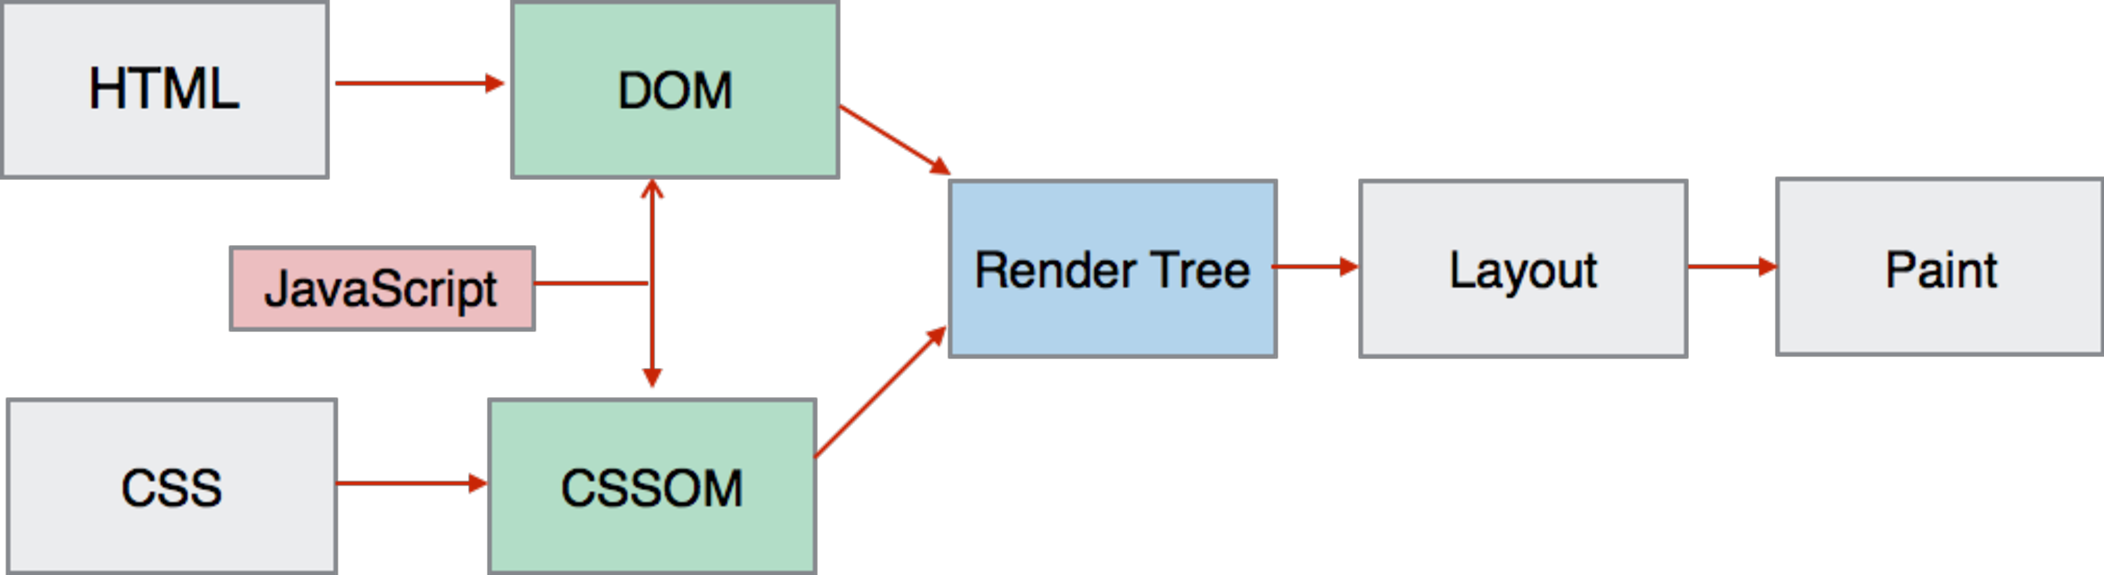
\includegraphics[width=0.85 \textwidth]{./figures/introduction/pageloadprocess.pdf}
  \caption {Page load process inside a browser}
  \label{fig:pageloadprocess}
\end{figure}

\noindent Browser starts off with fetching the html page (Figure \ref{fig:pageloadprocess}), a network activity. After receiving the first chunk of HTML page, HTML parsing process starts in parallel to generate the Document Object Model, or DOM\cite{dom}, a computation process.\\
DOM provides a structured representation of the document as a tree and it defines a way that the structure can be accessed from programs so that they can change the document structure, style and content.\\
\noindent  For example, for the sample following HTML code, first, the browser identifies HTML  {\em objects} such as {\em html}, {\em head}, {\em body} , \ldots.\\
\noindent Then, since the HTML markup defines relationships between tags, objects are connected in a tree data structure to hold the parent-child relationship from the original markup. {\em html} object is parent of the {\em body} object, the {\em body} object is parent of the {\em paragraph} object and so on.
\begin{minted}[frame=leftline, framerule=1.5pt, rulecolor=\color{blue}]{html}
<html>
  <head>
    <link href="style.css" rel="stylesheet">
  </head>
  <body>
    <p>Hello DOM!</p>
    <div><img src="d.jpg"></div>
  </body>
</html>
\end{minted}

\noindent The corrosponding DOM tree is depicted in figure \ref{fig:dom}.
 \begin{figure}[!htb]
  \centering
    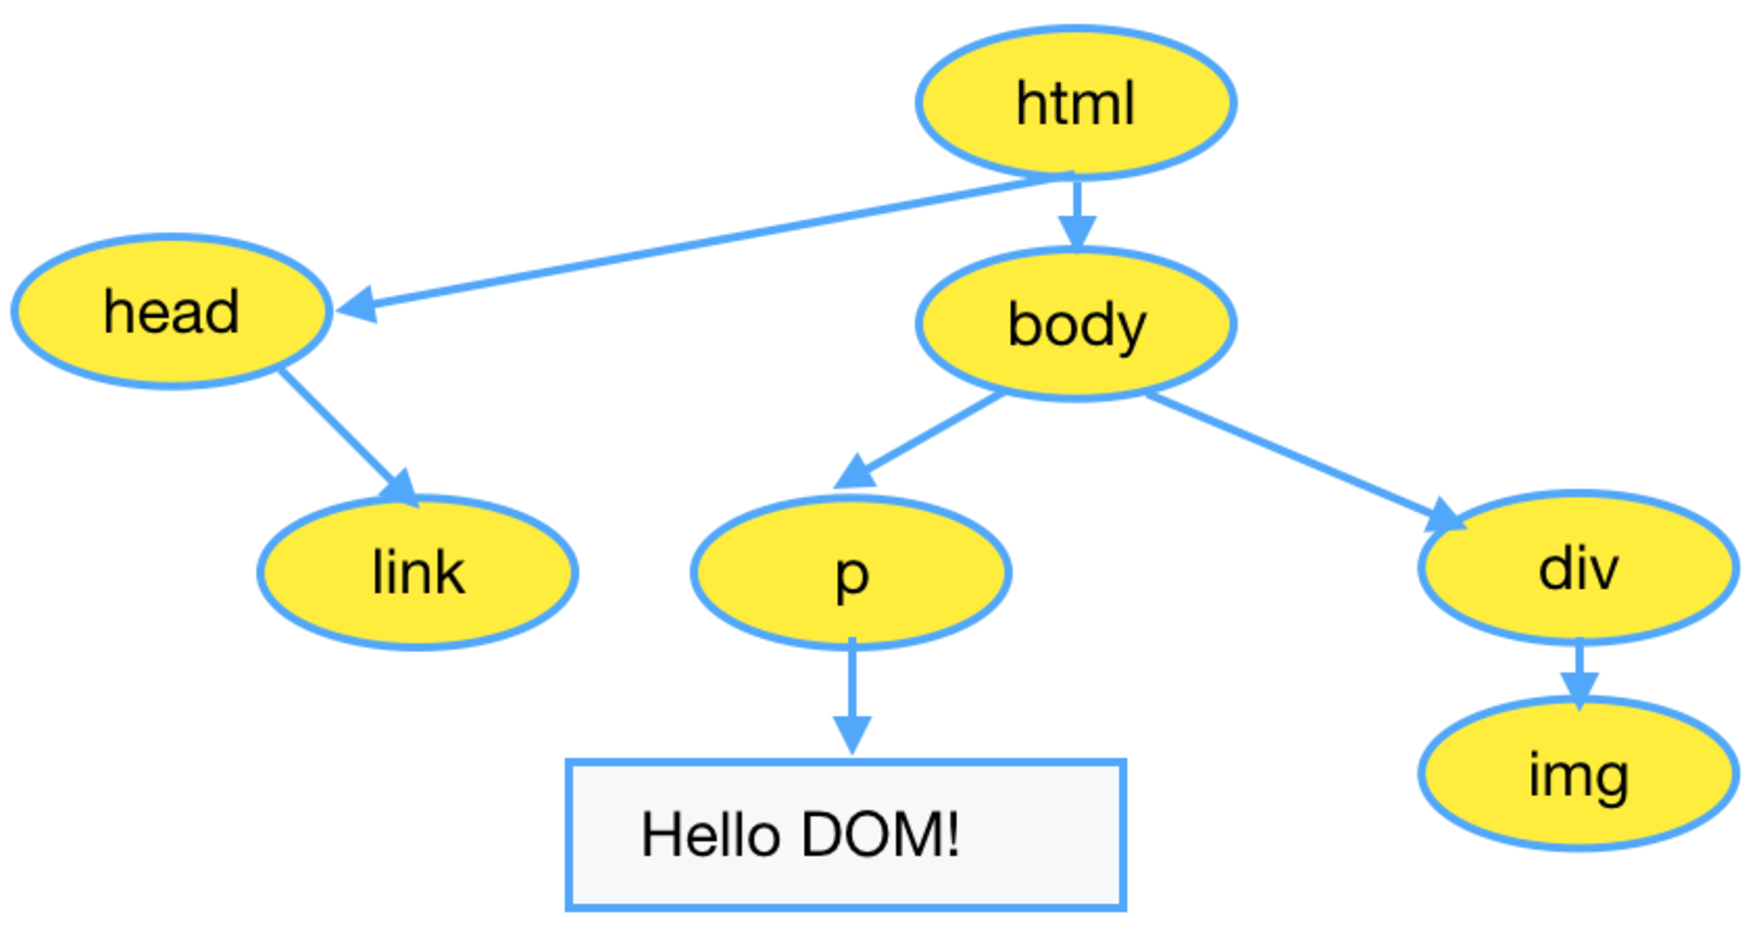
\includegraphics[width=0.85 \textwidth]{./figures/introduction/dom.pdf}
  \caption {DOM construction}
  \label{fig:dom}
\end{figure}

\noindent Rendering process also continuously renders the page, based on the intermediate DOM structure.
In rendering process, layout computes the exact position and size of each object and paint process takes in the final render tree and renders the pixels to the screen.\\

\noindent As the parsing progresses, new objects need to be downloaded based on the page's HTML code. If the object happens to be a regular Javascript (instead of asynchronous Javascript) or a CSS file, DOM construction process is blocked until these scripts are downloaded and parsed, Imposing {\em dependency} between activities.


\subsection{Dependency}
We start with {\em dependency} as the first challenge in improving page load time.
Each computation or networking elements running during the page load process is called an activity. 
As we have seen so far, activities lie in either {\em computation} or {\em networking} class. \\

\noindent From a different perspective, We can classify activities based on their dependency behavior.

\noindent There are activities that can be loaded/executed independent of  other activities\footnote{Obviously, all activities are dependent on the loading and parsing of the main html file. When we talk about activities, we are often talking about objects inside the root html file.}. \\

\noindent For example, two images in the following HTML code can be downloaded in parallel. Loading one of them does not depend on loading the other.\\ 


\begin{minted}[frame=leftline, framerule=1.5pt, rulecolor=\color{blue}]{html}
<html>
  <body>
     <img src = "a.jpg"/>
     <img src = "b.jpg"/>
  </body>
</html>
\end{minted}

\noindent In order to observe how activities are ordered in a page load process, We use WProf\cite{wprof}. WProf is discussed in \S\ref{ch:methodology}.
%WProf is a tool built atop the open source Chromium browser and is able to infer dependency policies of the browser. 
%WProf uses fine-grained timing of activities involved in a page load process to accurately extract the page {\em dependency graph} and the {\em critical path} inside such graph.
%We say an activity $a_2$ is dependent on a previously scheduled activity $a_1$ , if $a_2$ can be executed only after $a_1$ is being executed or completed. \\
%Considering activities as nodes of a graph  and inter-dependency relations as the edges of such graph, the resulting graph would be a DAG (Directed Acyclic Graph) which we call {\em dependency graph} hereafter.\\

%\noindent {\em Critical path} is the sequence of activities which add up to the longest overall duration inside the dependency graph.\\

%\noindent In addition, we use WProf-M, the mobile version of WProf for Android OS, to extract the dependency graph in a mobile environment.
\noindent For example, for the above mentioned HTML code, figure\ref{fig:twoimages} illustrates the corresponding dependency graph.\\
The X axis shows time in milliseconds and Y axis which grows from top to down, only  shows the order of objects inside an HTML file.
The light blue circle is the very first download HTML activity which is followed by a HTML evaluation activity (dark blue).
Two long purple bars refer to download of "a.jpg" and "b.jpg" ,respectively. 

 \begin{figure}[!htb]
  \centering
    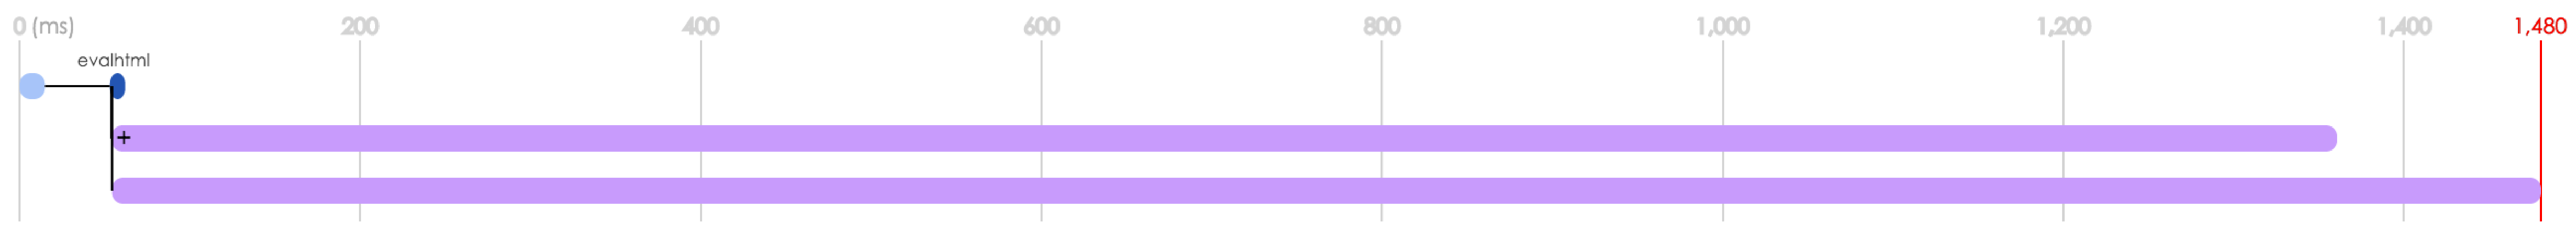
\includegraphics[width=0.85 \textwidth]{./figures/introduction/twoimages.pdf}
  \caption {Dependency graph for a HTML page with two independent images}
  \label{fig:twoimages}
\end{figure}

\noindent On the other hand, there are several activities inside a page load process that {
\em affects/will be affected} by other activities. 
For instance, adding more activities to the simple HTML code, brings about two different possible dependency scenarios:
\begin{enumerate}
  \item Adding Javascript after loading all images. 
   \begin{minted}[frame=leftline, framerule=1.5pt, rulecolor=\color{blue}]{html}
  <html>
  <body>
    <img src = "a.jpg"/>
    <img src = "b.jpg"/>
    <img src = "c.jpg"/>
    <img src = "d.jpg"/>
    <img src = "e.jpg"/>
    <img src = "f.jpg"/>
    <img src = "g.jpg"/>
    <img src = "h.jpg"/>
    <img src = "i.jpg"/>
    <script src = "b.js"> </script>
  </body>
</html>
\end{minted}
  In this case, as Javascript is loaded and executed after all images, image loading is not blocked by Javascript load, that is,  loading of images does not {\em depend} on loading of Javascript code.
  
However, there still is an internal dependency between loading the Javascript and it's execution.\\

Generally speaking, for all activities which need computation, such as HTML, Javascript, CSS, \dots  there always exists a {\em Load dependency}.
The dependency graph for this scenario is depicted in Figure\ref{fig:imagejs}\\ 
The bottom bars are showing Javascript ({\em b.js}) download and execution. They start after all images has been started.
 
 \begin{figure}[!htb]
  \centering
    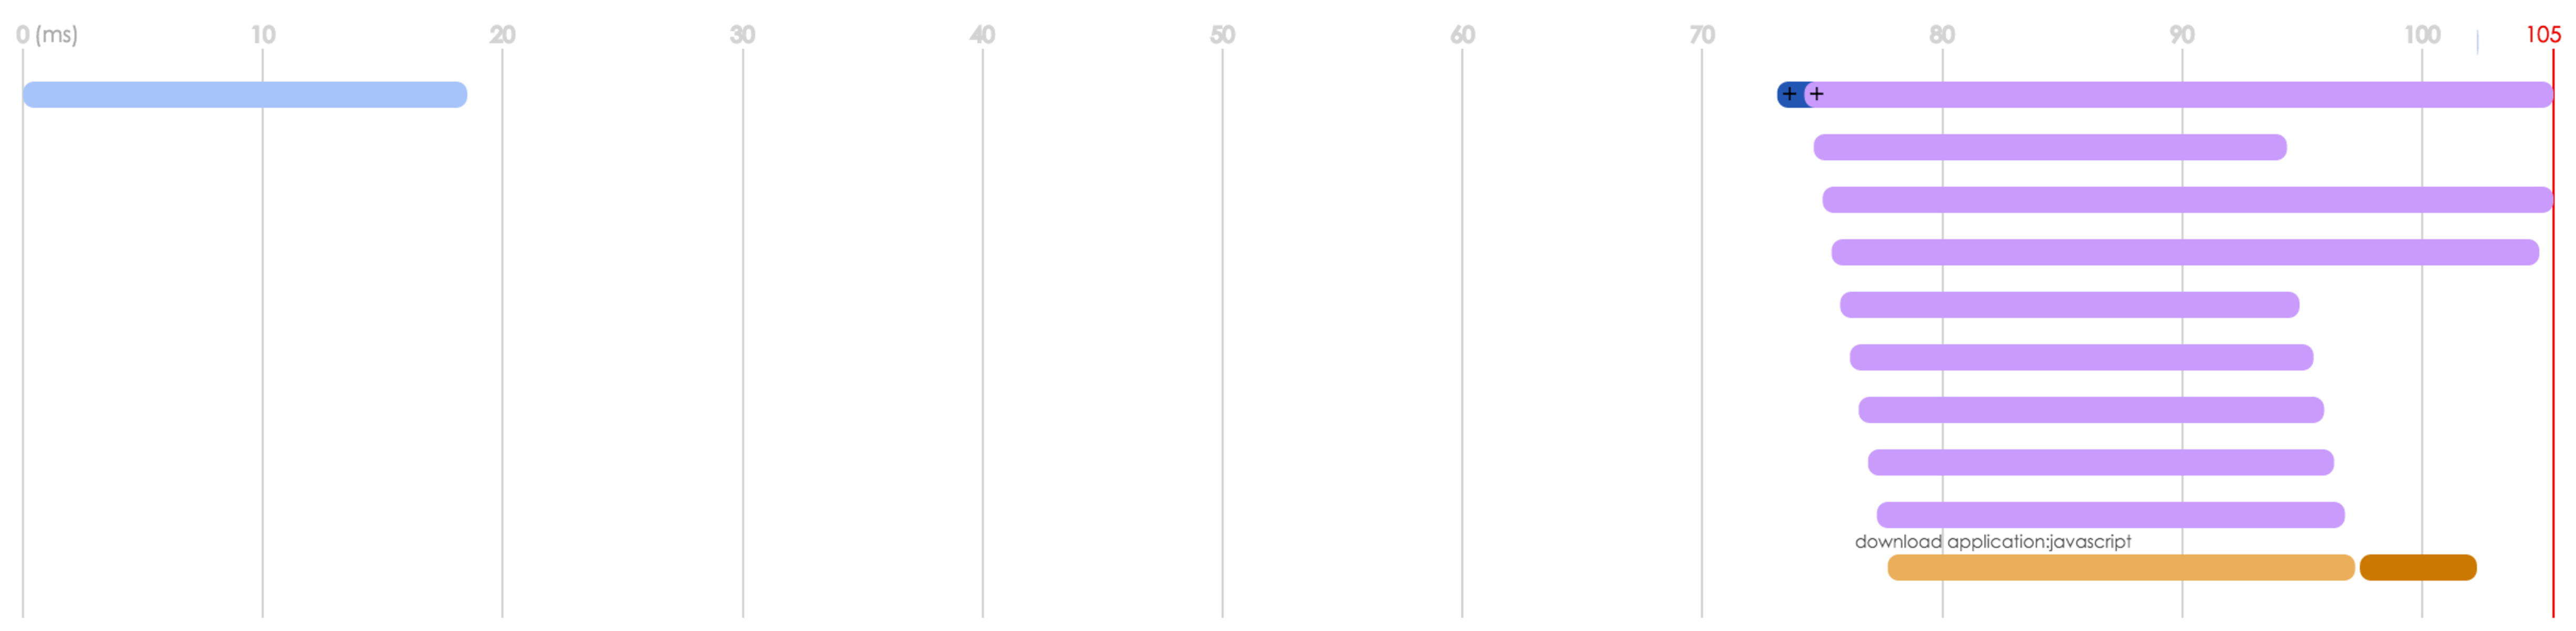
\includegraphics[width=0.85 \textwidth]{./figures/introduction/imagejs.pdf}
  \caption {Dependency graph for a HTML page when Javascript is loaded after all images}
  \label{fig:imagejs}
\end{figure}


  \item Adding Javascript before image load. 
  
  The interesting case is when Javascript code is located before images' ones.
  In this case, when the HTML parser encounters a dynamic activity that needs to be computed and is likely to modify the DOM tree. Browsers block subsequent activities until the dependency relations used in constructing the DOM tree are resolved. 
 If the dynamic activity does affect subsequent activities, It has to be loaded and computed before upcoming ones. 
 
However, in cases where parser realizes that this dynamic activity has no effect on download of subsequent ones, subsequent activities can be safely downloaded shortly after the execution starts .
 
The dependency graph for this scenario is depicted in figure\ref{fig:jsimage}\\
The top bars on the right are showing Javascript ({\em b.js}) download and execution which start before image loads.

  \begin{minted}[frame=leftline, framerule=1.5pt, rulecolor=\color{blue}]{html}
  <html>
  <body>
    <script src = "b.js"> </script>
    <img src = "a.jpg"/>
    <img src = "b.jpg"/>
    <img src = "c.jpg"/>
    <img src = "d.jpg"/>
    <img src = "e.jpg"/>
    <img src = "f.jpg"/>
    <img src = "g.jpg"/>
    <img src = "h.jpg"/>
    <img src = "i.jpg"/>
  </body>
</html>
\end{minted}

 \begin{figure}[!htb]
  \centering
    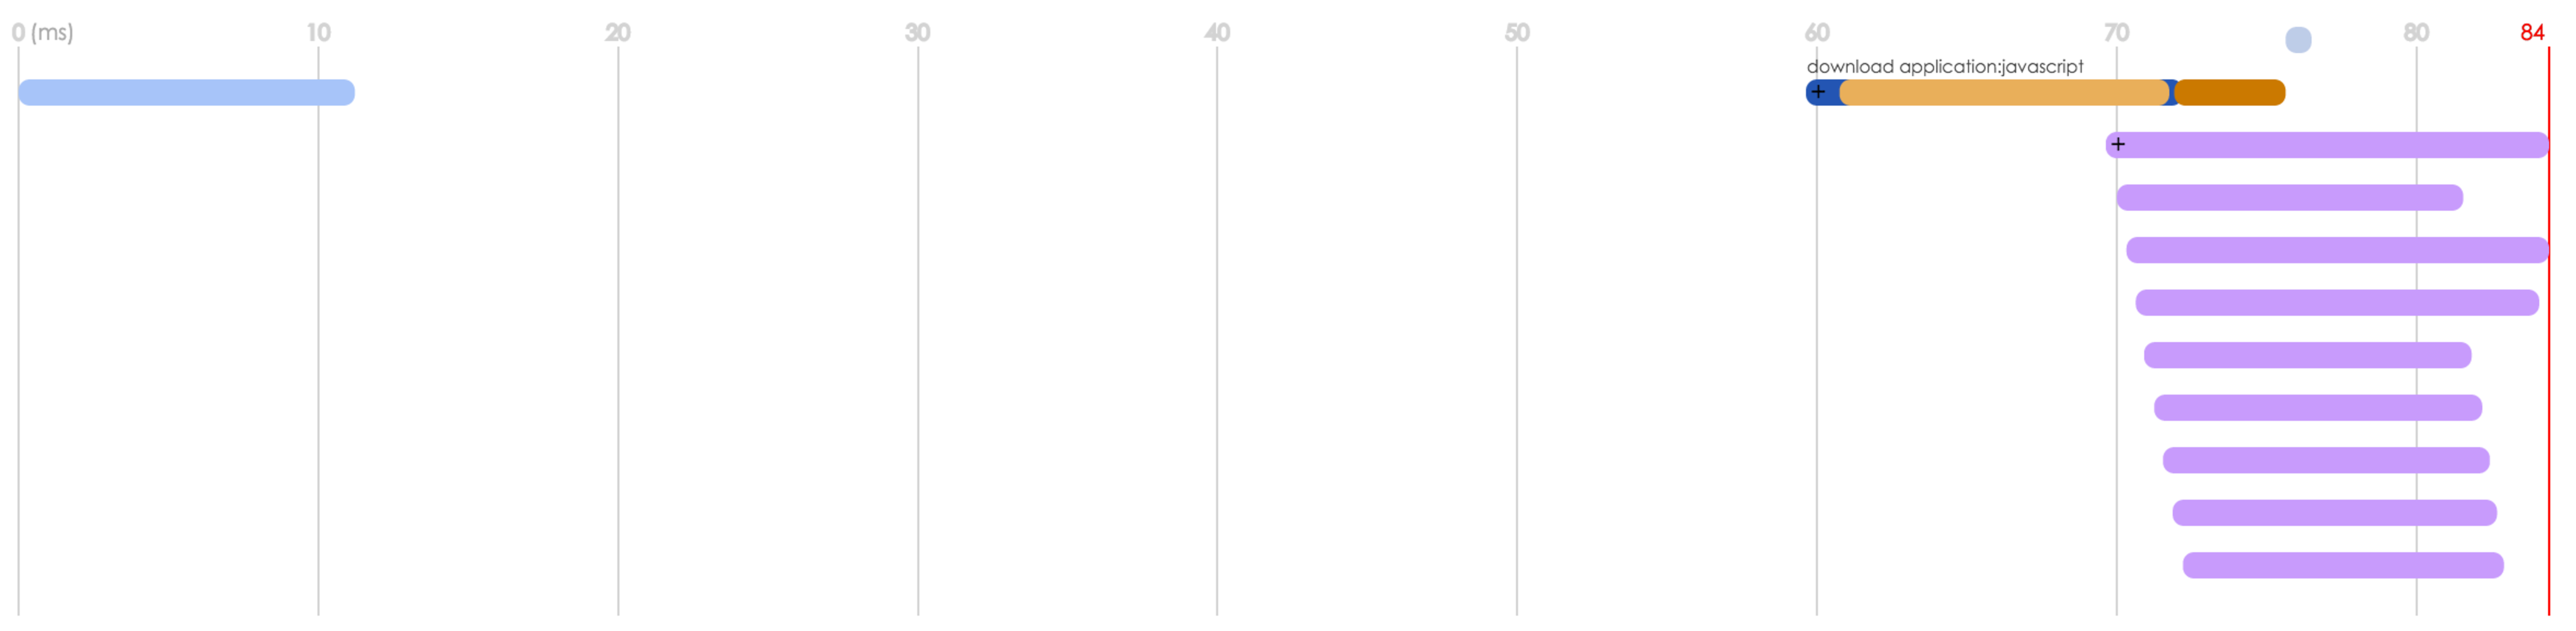
\includegraphics[width=0.85 \textwidth]{./figures/introduction/jsimage.pdf}
  \caption {Dependency graph for a HTML page when Javascript is loaded before images}
  \label{fig:jsimage}
\end{figure}

\end{enumerate}
 We can observe, if we reorder javascript and image locations in an HTML file, the resulting page and consequently the page load time is different.\\
 
\noindent \colorbox{gray!20}{\parbox{0.9\textwidth}{In other words, the performance, depends directly on how the dependency graph between markup, stylesheets, and Javascript is resolved}}

\subsection{Complexity}
The second challenge in improving page load time that we will look into is complexity.
Complexity of a website can be characterized as the number of objects inside it. \\
Adding more objects to a web page structure, not only increases the total size (which naturally means more download and computation time), but also has an effect on complexity of the dependency graph. \\
For instance, adding a Javascript to a page structure, spontaneously imposes one dependency between downloading and execution of that Javascript. Moreover, since Javascript modifies the DOM tree, all subsequent activities need to be blocked until the dependency issues are resolved. 

\noindent In figure \ref{fig:websitegrowth}, each X axis ticks corresponds to a year (J-95 for January 1995) and the right Y axis shows average number of objects for all website analyzes in that particular year.
We can observe that average number of objects in a webpage has doubled in last 7 years. 
The figure \ref{fig:websitegrowth} also shows that size of websites has doubled in only 3 years and 
Although computation power and network bitrate are also increasing, but we are dealing with an ever increasing trend in page size and the average number of objects in a web page. \\

\noindent \colorbox{gray!20}{\parbox{0.9\textwidth}{Increased size and number of objects, in turn, actuates the dependencies inside the page structure.
These all makes improving page load time even more complicated.}}

\begin{figure}[!htb]
  \centering
    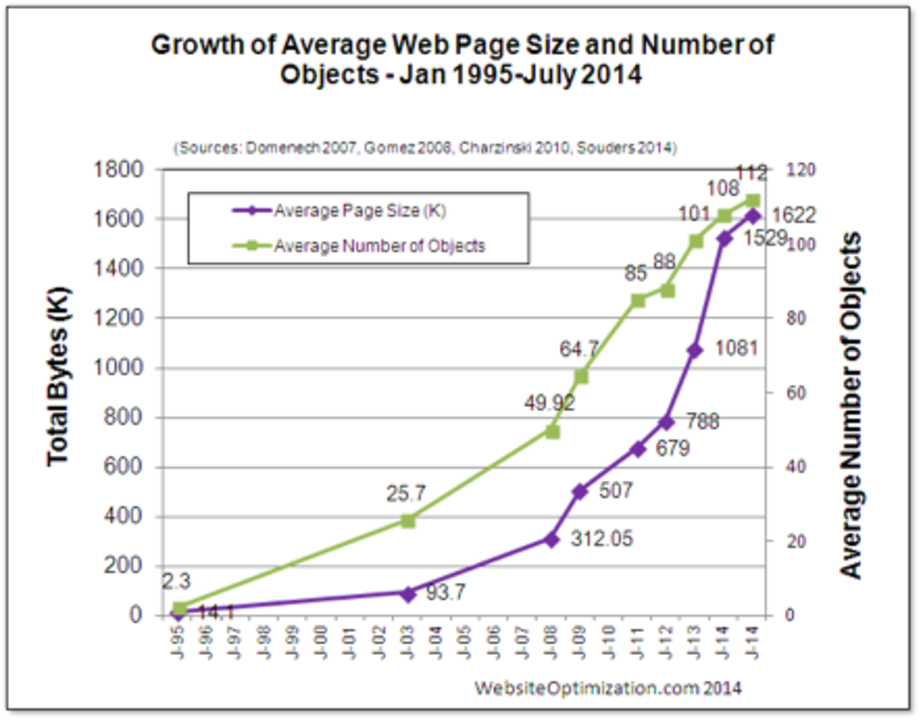
\includegraphics[width=0.75 \textwidth]{./figures/introduction/websitegrowth.pdf}
  \caption {Websites' size and objects growth (source: websiteoptimization.com)}
  \label{fig:websitegrowth}
\end{figure}
\subsection{Variances}
Another challenge that makes studying page load time complicated, is the variability of page load time over wireless/cellular networks. Page load time depends on several factors such as:
\begin{itemize}
\item Underlying network parameters including bandwidth, delay and packet loss.
\item Connection Type can be Wi-Fi, 4G, 3G, \dots, each with different characteristics.
\item Device computation and network resources such as CPU, RAM, wireless chipset,  \dots
 \item Even time and location of access may have effect on quality of network service one receives.
\end{itemize}

\noindent \colorbox{gray!20}{\parbox{0.9\textwidth}{Taking into account all these parameters is not a trivial task.}}

\section{Overview}\label{overview}
%Our goal is to improve Web sites' page load time on mobile devices. We will approach this goal by providing a framework for Web developers that suggest them best optimization applicable to their web sites.
Our primary object is to improve Web page load times. Although there are several approaches to improve Web pages, we propose the following: We will design algorithms and techniques to determine the best optimization(s) for a given page. Our goal is to provide an optimization framework for Web developers that will quickly suggest the best optimizations for a page.

\noindent The remainder of this report is organized as follows.\\
\noindent In order to address dependency and variances challenges, we start off by building a testbed to run our experiments in a controlled environment.
This testbed resolves the variances issue and lets us focus on each varying factor one at a time. (chapter \ref{ch:methodology})\\

\noindent Using the testbed, we first study the characteristics of the mobile page load process. From the experiments ran on this testbed, we observe that although networking time is the main bottleneck in desktop environment, but in mobile environment, main bottleneck in a page load process is the computation time. (chapter \ref{ch:bottleneck})

\noindent However, most mobile optimizations today including FlyWheel\cite{flywheel}, Parcel \cite{parcel}, HTTP/2 \cite{spdy}, attempt to reduce the network latency during page load time. 

\noindent Our dependency graph and critical path analysis approach using this testbed, enables us to study page load time behavior when a certain optimization is applied into a page structure (such as inlining) or when we change the way browsers and servers communicate (for example, enabling compression on server side).\\
\noindent Then, we will employ these findings to build a platform (PLTSpeed, our current project) to suggest users, what optimizations they need to apply and what is the effect of applied optimizations on their page's load time. (chapter \ref{ch:optimization})\\
\noindent In future, we propose to design and build a platform to predict page load time in a fast and scalable manner. Then, using this prediction mechanism, we suggest to users optimization (or an ordered list of optimizations) that most improve their Web site's page load time.\\

%\noindent . (chapter \ref{ch:pltspeed})





%\let\cleardoublepage\savecleardoublepage
%!TEX root = ../main.tex
\chapter{Related works}\label{ch:relatedworks}
In this chapter, we investigate previous efforts related to our work.
We start by studying other similar testbeds. Then we  explore proposed page load time improvement techniques, whether they are client side, server side or industry tools. We wrap up this chapter by looking into notable measurement studies related to our work.
\section{Testbeds}
\textbf{Mahimahi} \cite{mahimahi} is a framework to record traffic from HTTP-based applications, and later replay it under emulated network conditions. Mahimahi highlights it's features in  3 main parts:
\begin{enumerate}

\item It takes into account the multi-server nature of a webpage (external linked objects). Mahimahi launches separate web server instances for each external server to better emulate how web objects are delivered to the browser. Their results show that lack of multi-server emulation yields significantly worse performance at higher link rates.

\item It employs linux network namespace feature to isolate TCP/IP interactions for each instance.

\item The design is modular in the sense that different shells can be put together to build different architectures (like Lego blocks). Mahimahi is structured as a set of UNIX shells: 
\begin{itemize}
\item RecordShell, allows a user to record all HTTP traffic for any process spawned within it.
\item ReplayShell, replays recorded content using local servers that emulate the application servers.
\item To emulate network conditions, Mahimahi includes DelayShell, which emulates a fixed network propagation delay. 
\item  LinkShell, which emulates both fixed-capacity and variable-capacity links.
\end{itemize}
\end{enumerate}

\noindent While we share using Linux network name space with Mahimahi, there are  some fundamental differences between Mahimahi and  our approach. \\
In our testbed, we mainly focus on studying the critical path, and therefore record the page load time at the object
level rather than at the HTTP level as Mahimahi does.\\

\noindent Also, we are using well-proven Linux's Traffic Control program instead of a new link emulation software.\\

\noindent In addition, site manipulation is easier in our testbed as we have the whole page structure locally. For example, we can easily minify scripts and replay the new modified version locally.\\

\noindent Moreover, our testbed supports real mobile access, while MahiMahi emulates mobile devices.\\

\noindent \textbf{WebProphet} \cite{webprophet} was one of the first works to discuss dependencies for desktop browsers. WebProphet extracts dependencies in desktop browsers, and treats all computational activities as a black box. WProf, improved over WebProphet by uncovering dependencies in both networking and computational aspects of page load. We are also using mobile version of WProf to study dependencies in a mobile environment.\\

\noindent Finally, there are measurement platforms such as WebPageTest\cite{webpagetest} and HTTP Archives \cite{httparchive} which allow researchers to perform Web page measurements from several vantage points. They provide measurement data from a large number of networks and devices. However, we still lack tools to directly compare the performance of desktop and mobile browsers, or analyze the critical path.

 \section {Page load time improvements}
 There has been number of proposals to improve page load time in mobile environment. They either incline toward server or client side.
  \subsection {Client side improvements}
Qian et al.\cite{webcaching}, study  mobile web cache implementations across a wide range of applications and browsers, using data collected both from a large cellular operator (AT\&T) as well as 20 real users over several months. They study the impact of redundant transfers and identify the key root cause being broken caching logic in many HTTP library implementations used by native apps.  The result is that 18\% to 20\%  of HTTP transfers are redundant and could be eliminated with correct caching implementations.\\
Their results show that there exists a big gap between the protocol specification and implementation on mobile devices, which leads to significant amounts of redundant {\em network} traffic.\\

\noindent Zhue et al. \cite{webcore} take a "hardware-level" optimization approach by proposing the {\em "WebCore"} , a general-purpose core customized and specialized for the mobile Web browsing workload, to achieve both energy-efficiency and performance improvements in mobile web browsing.\\
 They aim to improve the {\em computation} part of mobile web browsing.
Their findings show that there are two main bottlenecks in current designs: Instruction delivery and data feeding.
{\em WebCore} adds two new components to the current CPU architecture:  Style Resolution Unit (SRU) and Software-Managed Browser Engine Cache.

\noindent Their results show that customizations alone on the existing general-purpose mobile processor design lead to 22.2\% performance improvement and 18.6\% energy saving.\\

 \noindent Wang et al.\cite{wang_www2012} add speculative loading to the current caching and pre-fetching solutions. In speculative loading, instead of trying to predict user behavior (pre-fetching), server's behavior is predicted.\\
Also, speculative loading starts loading the resources only after the user requests a webpage's URL in contrast to prefetching that loads the resources beforehand.\\
In their experiments, they observe on average, 76\% of the resources in one webpage are shared by at least one other webpage from the same website. Hence, they conclude that after a user visits a website for enough times and the resource graph is constructed, the browser can potentially predict the majority of the sub-resources (mostly CSS and Javascript) needed for a new webpage visit, and thus speculatively load them.\\

\noindent On their experiments they observed a maximum of 1.4 seconds improvement in page load time and consider this as a limit for any client-only solution.\\
However, they consider network RTT as the major bottleneck in mobile browser performance . %This may make sense as this paper was written in 2012 (The RTT of typical 3G network is around 200 ms) but the result may not hold any more.
 
 \subsection {Server side improvements}
Sivakumar et al.\cite{cloud_hotmobile2014} compare CB (cloud based) with Direct (device based) mobile browsing and how they affect page load time and total energy. 
In a CB, all or part of the computation or netwoorking tasks are offloaded to the cloud, while in Direct, every thing is done on the client device.
By using CB, mobile device can offload heavy processing components such as JavaScript to the cloud in order to reduce CPU time and energy. Then the processed page is returned in a specific notation (Called CBML: Cloud Based Markup Language) to the mobile device. \\

\noindent Another benefit of using CB is data compaction performed in cloud which aims to decrease page load time and transferred bytes.
Their evaluations indicate that neither Direct nor CB is better under all scenarios. For e.g. while CB decreases the download time compared to Direct for 38.87\% of pages, it increases it by as much as 29.8s for other pages. Similarly CB increases energy usage by up to 21.31J compared to Direct for some pages.
They have found root causes of these variances to be: Extent and duration of Javascript run in the page and compaction ratio.\\

\noindent PARCEL\cite{parcel} moves the task of identifying and downloading objects needed to render a Webpage to a proxy. Main focus of PARCEL is to support cellular friendly data-transfers by reducing the number of HTTP request-response interactions. Unlike {\em cloud based browsing} \cite{cloud_hotmobile2014}, PARCEL keeps most other functionalities including Javascript execution in the client browser and does not try to offload the {\em computation} part.
PARCEL uses it's own browser to communicate with the proxy part and therefore is more of a mixed (client and server) solution.\\

\noindent FlyWheel\cite{flywheel} is Google's data reduction proxy service that provides an average 58\% byte size reduction of HTTP content. FlyWheel also focuses  on {\em network} bytes transfer. Overhead of compression and decompression on CPU time and energy consumption has not been studied in FlyWheel.\\

\noindent KLOTSKI\cite{klotski} states that "the increasing complexity of web page content and decreasing user tolerance will outpace the benefits from incremental performance enhancements such as compression, caching, cloud based browsers, \ldots". Therefore, they focus on improving user experience, instead of decreasing total page load time. In order to do that, they propose a platform which dynamically reprioritizes web content so that the resources on a page that are critical to the user experience are delivered sooner.
To respond to a request, KLOTSKI first selects the subset of resources on the page that it should prioritize. Thereafter, as the client executes the page load, the front-end alters the sequence in which the page's content is delivered to the client, in order to prioritize the delivery of the selected subset of resources.\\
 \subsection {Industry tools}
Google's PageSpeed Insights \cite{pagespeedinsight} is a tool that analyzes web pages and generates tailored suggestions to make the pages faster. PageSpeed Insights analysis does not use real devices, instead it changes the user-agent for desktop and mobile in webkit renderer accordingly.

\noindent PageSpeed Insights uses a set of predefined rules to evaluate a webpage. Each PageSpeed rule generates an impact number that indicates the importance or priority of implementing the rule-result suggestions for the rule, relative to other rules. \\
 
\noindent YSLOW \cite{yslow} is Yahoo's performance analysis tool that grades a web page, based on one of three predefined ruleset or a user-defined ruleset. It also offers suggestions for improving the page's performance.\\

\noindent Neither PageSpeed Insights nor YSlow metrics, directly indicate page load time. Part of our current project is defining a new scoring system that is correlated with page load time and shows amount of improvement based on the page load time improvement.\\


\section{Measurement studies}
Qian et al. \cite{qian_mobisys2014} provide a comprehensive measurement study to  examine  the resource usage of mobile browsers, but mainly focus on cellular bandwidth and energy usage rather than computation and page load times.\\

\noindent Bui et al. \cite{bui2015rethinking} propose techniques to optimize the energy consumption of web page loading on cellphones.
Their network-aware resource processing and adaptive content painting, aim to address energy inefficiency issues of the current mobile web browsers in its content processing and graphic processing pipelines.\\
Application assisted scheduling's goal is  to balance the trade-off between the energy saving and the QoS in ARM's big.LITTLE platforms.\\
However, their focus is more on lowering energy consumption, without affecting the original page load time.\\

\noindent Singh et al. \cite{singh2015flexiweb} show that compression middleboxes are not always helpful. Compression middleboxes are middle servers that compress page content and are usually deployed as part of a content delivery network.
commonly used today. 
 They observe from extensive measurements that the compression middle-box should be used only when network conditions are bad and otherwise, should be directly fetched from the original web server. 
Based on this observation, they build FlexiWeb, a framework that supports network-aware middle-box usage. In addition, FlexiWeb  performs dynamic network-aware compression to provide further performance gain.\\

\noindent Butkiewicz et al. \cite{butkiewicz2011understanding} characterize Web page complexity.
They show a website's popularity is not a good indicator of its complexity, whereas its category does matter. For example, {\em www.google.com} is a popular website but not a complex one.
They have also found news sites load more objects from more servers and origins than other categories. Their analysis show that number of objects and number of servers are the dominant indicators of page load time and variability in page load times, respectively.\\

%{\em What about moving this to complexity part? As a good reasoning why complexity is important}.

\noindent Wang et al. \cite{spdy_nsdi} show that although SPDY has been designed to decrease transfer time because of it's use of a single TCP connection, but this feature is also detrimental under high packet loss.






%!TEX root = ../main.tex
\chapter{Design and Methodology}\label{ch:methodology}
%There are two main requirements to build a dependency graph and critical path analysis testbed. 
%First, we require tools to perform critical path analysis on mobile page loads, to determine the bottlenecks. Second, we need to design an experimental testbed that will allow us to perform comparison studies in the presence of large variances.
To overcome challenges addressed in \S\ref{ch:introduction}, we design and build our own testbed.
To address {\em dependency} challenges, we use WProf \cite{wprof} which takes into account internal page dependencies and to address high {\em variances} in a page load process, we provide a controlled environment to run our experiments.
\section{WProf}
WProf is a tool built atop the open source Chromium browser and is able to infer dependency policies of the browser. 
WProf uses fine-grained timing of activities involved in a page load process to accurately extract the page {\em dependency graph} and the {\em critical path} inside such graph.
We say an activity $a_2$ is dependent on a previously scheduled activity $a_1$ , if $a_2$ can be executed only after $a_1$ is being executed or completed. \\
Considering activities as nodes of a graph  and inter-dependency relations as the edges of such graph, the resulting graph would be a DAG (Directed Acyclic Graph) which we call {\em dependency graph} hereafter.\\

\noindent {\em Critical path} is the sequence of activities which add up to the longest overall duration inside the dependency graph.\\

\section{WProf-M} To perform critical path analysis on mobile devices, we use a version of WProf on Android Chromium Version 31.0.1626.0. As a first step, we repeat our browser instrumentation experiments on mobile browsers to infer the dependency policies on the Android Chromium browser. To infer dependency policies in networking loading and computational activities, we load carefully crafted test pages. The set of Web pages we use to infer the dependency policies can be found at \url{wprof.cs.washington.edu/tests/}. \\

\noindent Next, we instrument the Android Chromium browser to record the timings of each page load activity and use the timing and the dependency policy to extract the dependency graph and compute the critical path.

\section{Testbed Design} One of the challenges in studying effect of an optimization on page load time is that Web page loads have high variance~\cite{spdy_nsdi}. The variance makes it non-trivial to isolate the performance of the mobile browser: if the page load times on the mobile browser is very different when an optimization is applied, the difference could be because of the optimization or because of page load variance.

\noindent We design an experimental testbed that minimizes variance when loading pages before and after optimizations. We make the following design choices:
 \begin{itemize}
  \item  We serve pages from the local server. To this end, we download the entire page locally on the server and convert all the external links to local links.  This minimizes variances caused by changes to the page. 
   \item When comparing mobile and desktop browsers, we load the same page on the mobile and the desktop browser, rather than loading the mobile version of the page (or {\em mpages}) to perform more direct comparisons.
    \item  We emulate different network conditions using a traffic controller to ensure that both the mobile and the desktop browser load pages under the same network conditions.
    \end{itemize}

\noindent To ensure that the results we get from our controlled setting applies more broadly, we perform additional experiments where the three restrictions are removed; i.e., we load pages directly from the Web server, we load {\em mpages}, and we use real networks. Our additional experiments show that the conclusions we derive from our controlled experiments also apply more generally. \\

 \begin{figure}[!htb]
  \centering
    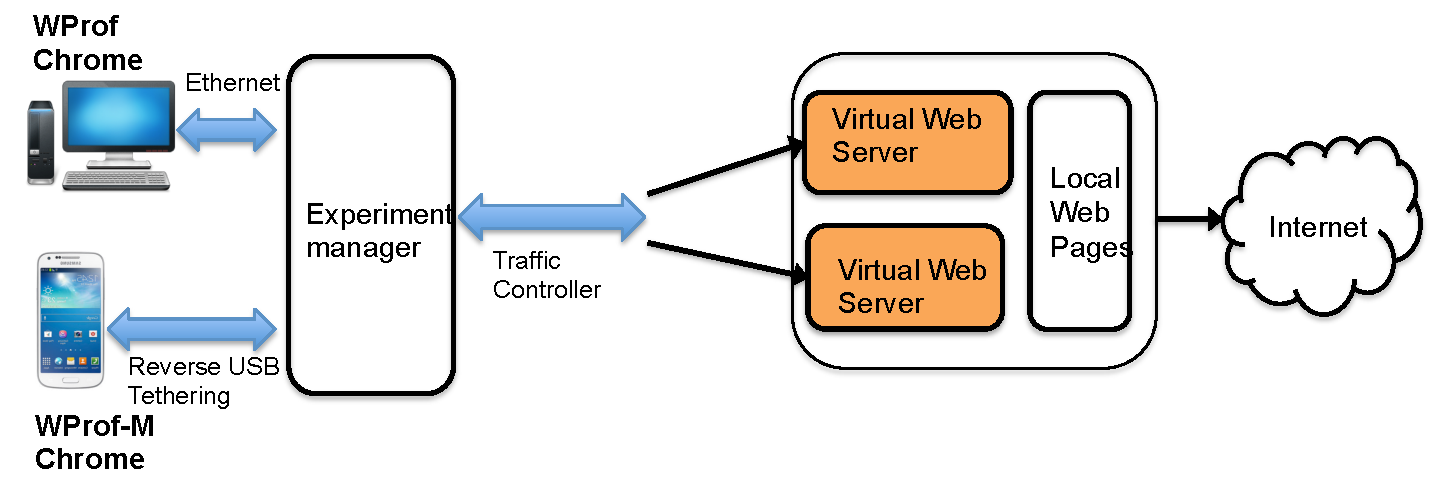
\includegraphics[width=0.9 \textwidth]{./figures/methodology/architecture.pdf}
  \caption{Testbed architecture}
  \label{fig:architecture}
\end{figure}

\noindent Figure~\ref{fig:architecture} shows our experimental testbed. At the client side, we load Web pages on a phone running Android Chromium instrumented with WProf-M, and on a desktop running WProf instrumented Chromium. All Web page loads go through the experiment manager. The manager stores logs generated by WProf and WProf-M and configures the traffic controller and the Web server if needed.  We use USB tethering to connect the mobile device to the experiment manager rather than connect using WiFi because we observed large variances in WiFi latencies.\\

\noindent On the server side, we leverage virtual machines to run multiple web servers on the same platform. To isolate the different network stacks for the difference virtual servers, we use Linux network namespace~\cite{namespace}, similar to \cite{mahimahi}.  To emulate different network conditions, we are using  Linux Traffic Control (TC). Before each experiment, we run ping and iperf tools to test that the emulated network has the expected bandwidth and delay values. 

\section{Parameters}
\label{sec:parameters}

The parameters used in our testbed are as follow\\

{\noindent {\bf Server and Client:}} All Linux instances are virtual machines running inside a VMware ESXi 6.0  Bare-Metal Hypervisor. On average, 4 cores at 2.6GHz and 2GB of RAM has been assigned to each virtual machine. \\

\noindent We use two Samsung Galaxy S4 phones running Android KitKat and Samsung Galaxy S6 phones running Android Lollipop. 
By default, we present experiments conducted on Samsung Galaxy S4 phones on the controlled testbed. \\

{\noindent {\bf Network:}} We run the emulated network experiments on 6 different network profiles under the following bandwidth: 1Mbps, 5Mbps and 20Mbps. We experiment with two round trip delays: 50ms and 150 ms. We inject up to 2\% packet loss rate based on real world studies~\cite{dukkipati_imc2011}.\\
   
 \begin{table}[!htb]
\centering

\begin{tabular}{|l|l|l|l|}
\hline
\rowcolor[HTML]{656565} 
{\color[HTML]{FFFFFF} {\bf }} & {\color[HTML]{FFFFFF} {\bf lab\_WiFi}} & {\color[HTML]{FFFFFF} {\bf lab\_3G}} & {\color[HTML]{FFFFFF} {\bf lab\_4G}} \\ \hline
Average                               & b20-d50                                  & b1-d50                                  & b5-d50                                  \\ \hline
Poor                                     & b20-d150                                  & b1-d150                                  & b5-d150                               \\ \hline
\end{tabular}
\caption{Different network profiles set up in testbed. b: bandwidth in each direction, d: round-trip delay time}
\label{table:net_profiles}
\end{table}

\noindent Table \ref{table:net_profiles} shows the different network profiles. Based on our lab experiments we categorize each pair of bandwidth and round trip delays as latencies seen in WiFi, 3G, and 4G networks.\\
   
{\noindent {\bf Webpages:}} We experiment with 200 Web pages. We randomly choose 40\% of the Web pages from the top 200 websites in Alexa~\cite{alexa}, 30\% from the pages from the bottom of Alexa's 1 million web sites, and the remaining 30\% from news websites on Alexa. We choose a mix of Web pages for the following reason: typically the popular top 200 Web pages on Alexa are smaller (for example, google.com) and are highly optimized. The performance of such Web pages may not be typical. Instead, we include unpopular pages in our mix because they are likely to not be  optimized.  We also choose news websites because they tend to be complex pages. \\

\noindent In the common case, we load the original page on both desktop and mobile. We  perform addition experiments where we load mobile version of the page, that we call {\em mpage}. For example,  \url{m.cnn.com} is an mpage, where the original page is \url{www.cnn.com}. Note that by default, mobile browsers always redirect to the {\em mpage}. We modify the user agent field to force the mobile browser to load the original page. We do this  to directly compare the performance differences between  mobile and desktop browsers.\\

{\noindent {\bf Metrics:}}

\noindent We measure page load  performance using the Page Load Time (PLT) metric. The Page Load Time metric is commonly defined as the time between when the page is requested and when the {\em DOMLoad} event is fired~\cite{wprof}. The DOMLoad event is fired when all  objects are
fetched, processed, and added to the DOM. There has been several alternate metrics to define page load performance such as the above-the-fold metric~\cite{aft}. However, these alternate metrics are not easy to compute and are not yet widely used. \\

\noindent For each page load, we  estimate the critical path. We divide the critical path into the following components:
\begin{itemize}
\item Computation: We sum the time taken by the following activities on the critical path: HTML Parsing, Javascript/CSS evaluation, and rendering. We call this the computational component of the critical path. 
\item Network: We sum the time taken to load each object on the critical path. 
\end{itemize}



%!TEX root = ../main.tex
\chapter{Characterizing bottleneck in mobile page load}\label{ch:bottleneck}
As discussed earlier in \S\ref{ch:introduction}, lots of parameters are involved in a page load process.
We also categorized activities involved in a page load, in two main classes: networking activities and computation activities.\\
In this chapter we start off by studying the importance of these two classes and observe how they effect the page load time.
Then, we will look into the critical path and how that would be affected in different situations.

\noindent Characterizing mobile page load times would be our first step towards improving page load performance.

\section{Computation is the bottleneck}

In this section, we show the results of experiments we have run under different network profiles for our set of Web pages, as discussed in \S\ref{sec:parameters}.
We test both desktop and mobile browsers and show the main bottleneck in a page load process.

Our main observations are as follows: 
\begin{itemize}
\item On mobile devices, when analyzing critical path, we observe that in almost all network profiles, ranging from  {\em average lab\_Wifi} to {\em poor lab\_3G}, computation time, rather than networking time, is the dominant factor in the whole page load time .
On contrary, on desktop browsers, networking time takes the majority of the page load time, independent of network profile.
\item Computation still continues to be the bottleneck even when we switch to the new Samsung Galaxy S6 phones, with better computation resources.

\item Computation is still bottleneck on mobile browsers when pages are loaded {\em in-the-wild}. i.e from the original Web server on real WiFi connections rather than in our controlled environment. 
\end{itemize}

\subsection{Page load times}

Figure~\ref{fig:plt_desktop_mobile_mpage} shows the page load times to load pages on desktop browsers, mobile browsers, and to load {\em mpages} on mobile browsers. These are the results of all Web pages and across all network profiles. We can observe that median of page load time on mobile browsers (both original pages and {\em mpages}) is two times greater than that of desktop's in the same network profile.
The difference in tail is much higher. We see later (\S\ref{sec:unrestricted}) that when loading pages on desktop browsers using Ethernet connection, the difference in page load time between mobile and desktop browsers is even higher.

\begin{figure}[!htb]
\centering{
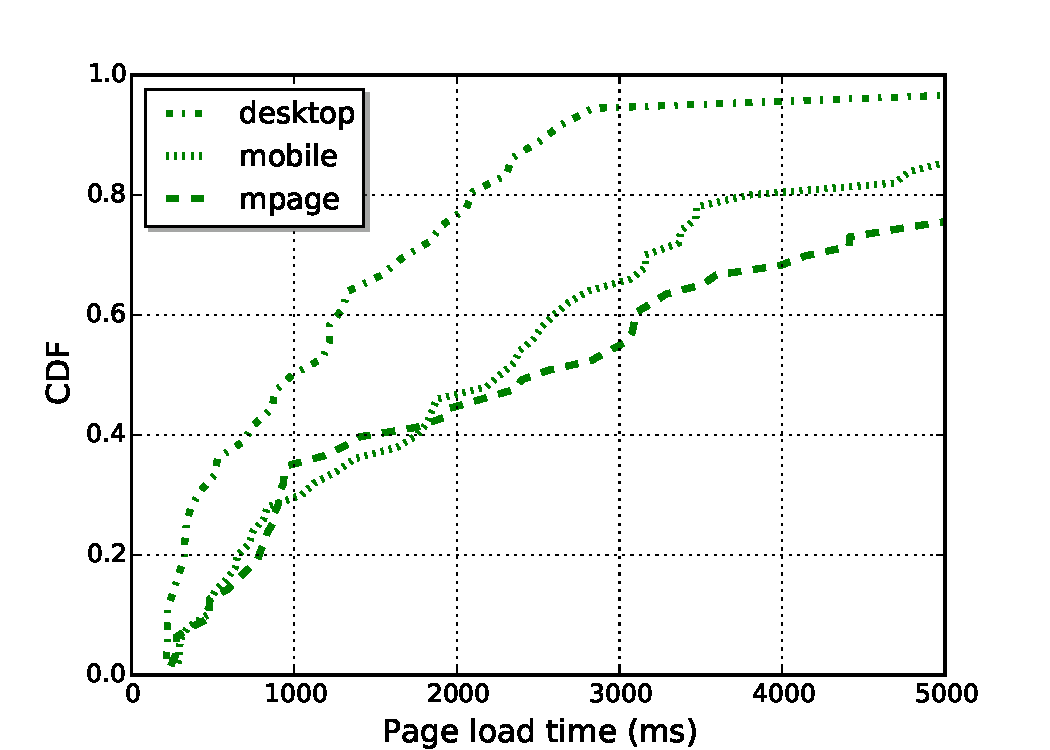
\includegraphics[scale=0.5]{./figures/plt/plt_desktop_mobile_mobileversion.pdf}
\caption{Comparing the page load times between loading original pages on mobile browser vs desktop browser, and loading {\em mpages} on the mobile browser.   }
\label{fig:plt_desktop_mobile_mpage}
}
\end{figure}

\noindent Although {\em mpages} are smaller versions of the original pages, we do not see a significant difference between page load times when loading original pages and {\em mpages} on mobile. Reducing object sizes, would directly affect the download time for those objects but does not necessarily reduce the computation requirement. %proportionally.

\subsection{Bottleneck in mobile vs desktop browsers}
In order to pinpoint the bottleneck in a page load process, we load the same set of Web pages on desktop ad the mobile browsers, under the same network conditions.
Figure~\ref{fig:comp_net_fraction_average} shows the fraction of computation activities on the critical path and the fraction of network activities on the critical path for desktop browsers. Figures~\ref{fig:non-mobile-b20-d50} and~\ref{fig:non-mobile-b5-d50} show that downloading objects takes 60\% of the total delay on the critical path, while the computation activities is responsible for only  40\% of the total delay on the critical path. This relation holds for different network profiles.

\begin{figure}[!htb]
    \begin{subfigure}{0.48\textwidth}
        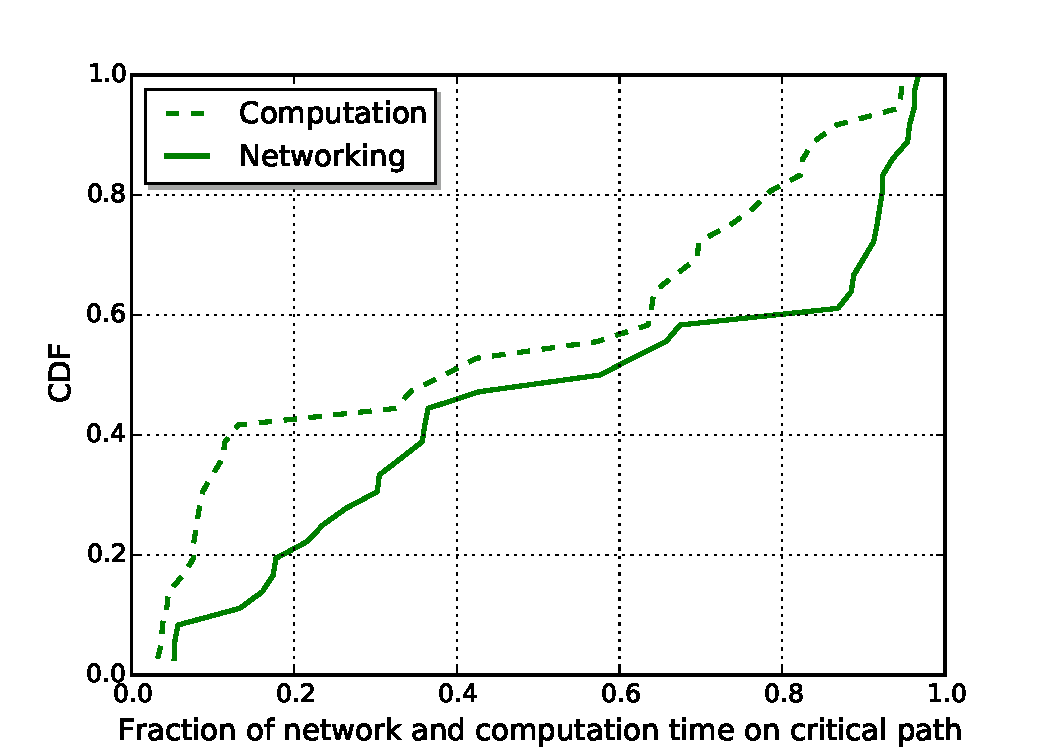
\includegraphics[width=1\linewidth]{./figures/computation/desktop-b20-d50.pdf}
        \caption{Desktop, Average lab\_Wifi}
        \label{fig:non-mobile-b20-d50}
    \end{subfigure}%
    \begin{subfigure}{0.48\textwidth}
        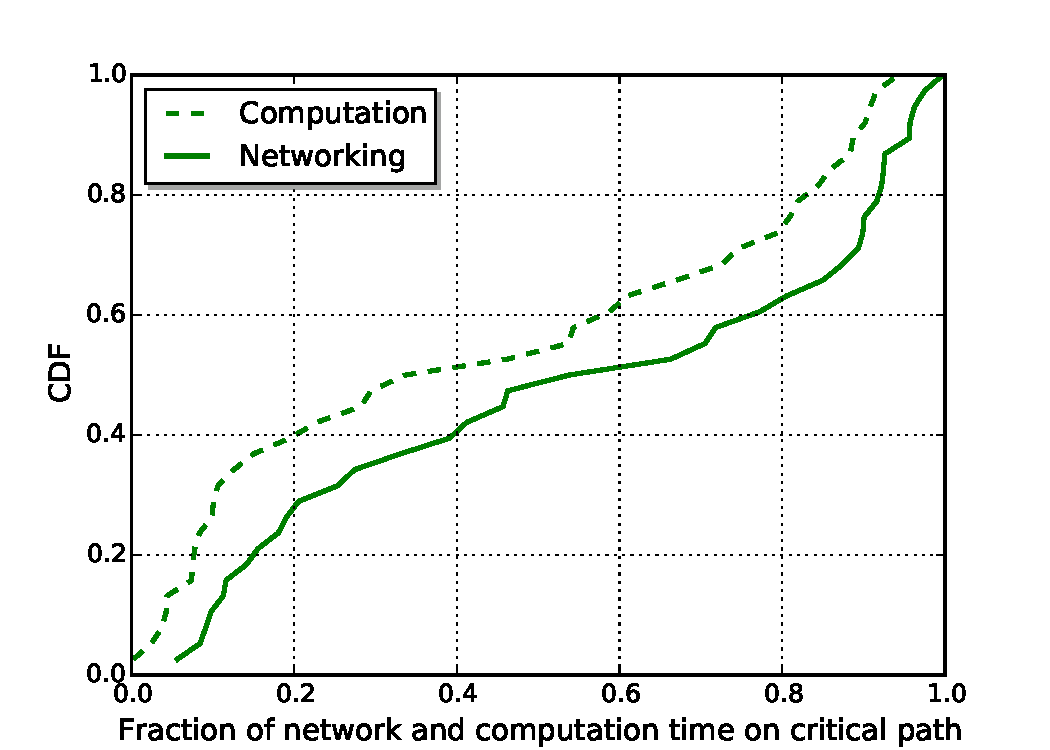
\includegraphics[width=1\linewidth]{./figures/computation/desktop-b5-d50.pdf}
        \caption{Desktop, Average lab\_4G}
        \label{fig:non-mobile-b5-d50}
    \end{subfigure}
   \begin{subfigure}{0.48\textwidth}
        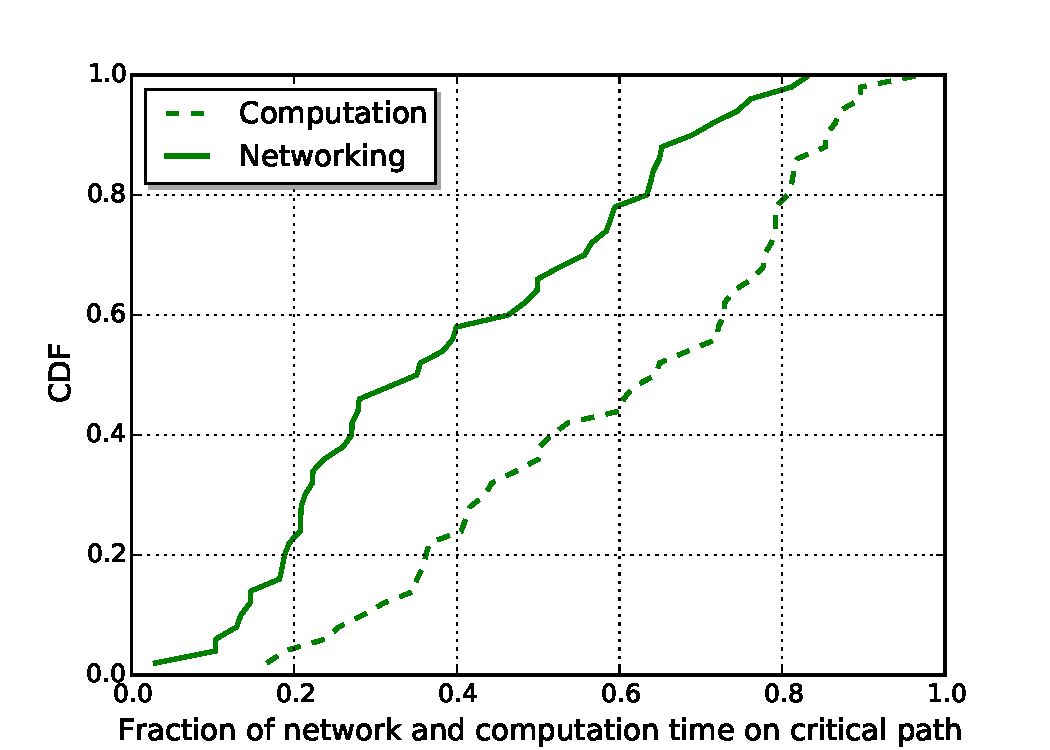
\includegraphics[width=1\linewidth]{./figures/computation/mobile-b20-d50.pdf}
        \caption{Mobile, Average lab\_Wifi}
        \label{fig:mobile-b20-d50}
    \end{subfigure}%
    \begin{subfigure}{0.48\textwidth}
    \centering
        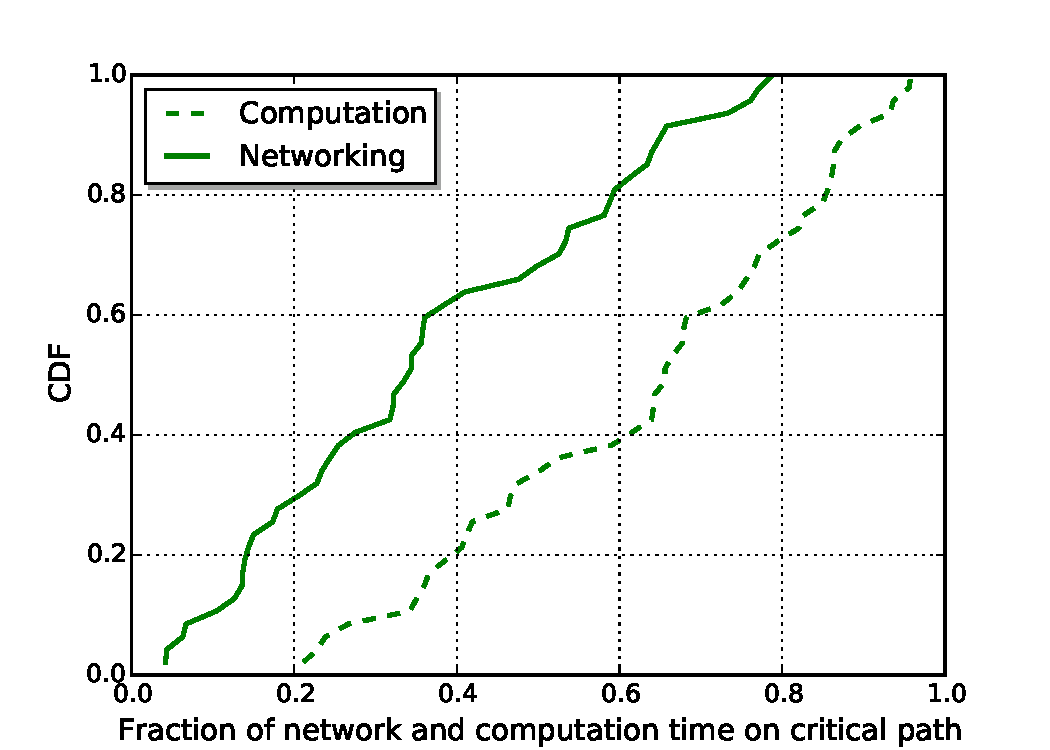
\includegraphics[width=1\linewidth]{./figures/computation/mobile-b5-d50.pdf}
        \caption{Mobile, Average lab\_4G}
        \label{fig:mobile-b5-d50}
    \end{subfigure}
      \caption{Average Wireless Connectivity: Fraction of network and computation time on critical path. Under average connectivity, computation is the main bottleneck for mobile browsers. }
    \label{fig:comp_net_fraction_average}
   \end{figure}
   
\noindent However, for mobile browsers computation time versus network activities time on the critical path  is different. Figure~\ref{fig:mobile-b20-d50} and~\ref{fig:mobile-b5-d50} shows that on both the average lab\_Wifi and the average lab\_4G networks, the bottleneck is the computation activities when loading a page on mobile browsers. Computation accounts for over 60\% of the page load time on the critical path in the median case when loading pages on mobile browsers. The results for the lab\_3G network is quantitatively similar (not shown here).

\noindent Figure~\ref{fig:comp_net_fraction_poor} shows the same bottleneck analysis but when the wireless network is of poor quality with longer round trip times of 150ms. Surprisingly, even when the network is poor, Figure~\ref{fig:mobile-b20-d150} shows that computation remains a bottleneck for page load on poor lab\_WiFi, accounting for 55\% of the page load time in the median case. It is only in the poor lab\_4G environment that the network becomes the bottleneck when loading pages on the mobile browser. On the other hand, on desktop browsers, poor wireless condition only makes the network bottleneck even more pronounced (Figures~\ref{fig:non-mobile-b20-d150} and~\ref{fig:non-mobile-b5-d150}).
\begin{figure}[!htb]
    \begin{subfigure}{0.48\textwidth}
        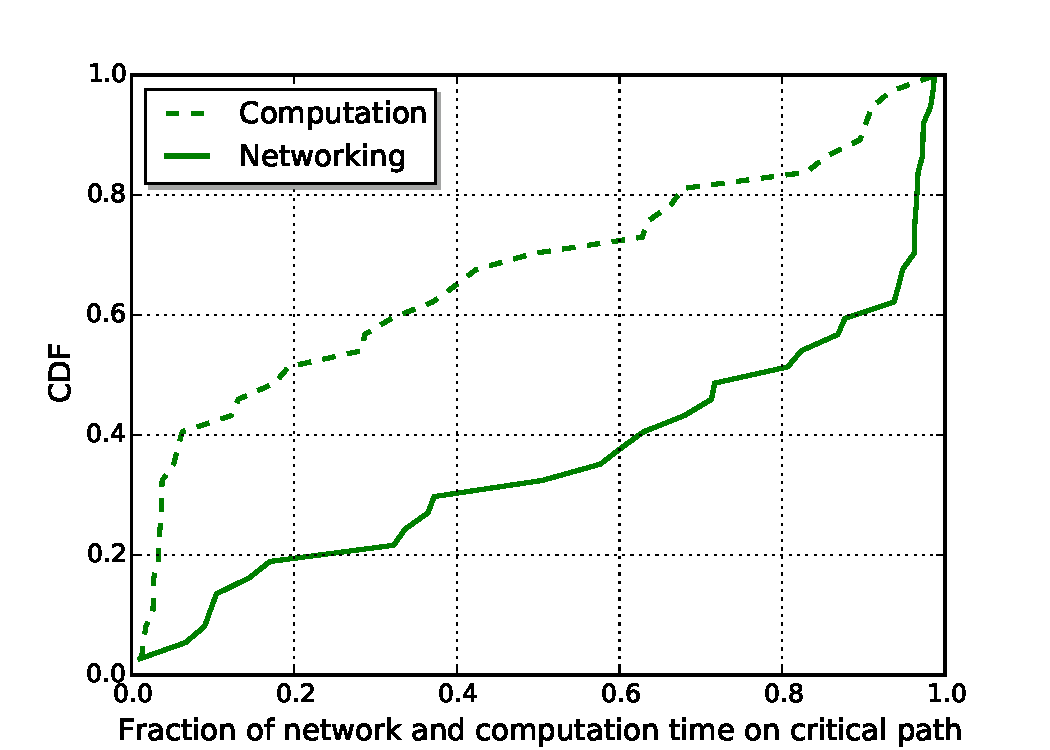
\includegraphics[width=1\linewidth]{./figures/computation/poor/desktop-b20-d150.pdf}
        \caption{Desktop browser, Poor lab\_Wifi}
        \label{fig:non-mobile-b20-d150}
    \end{subfigure}%
    \begin{subfigure}{0.48\textwidth}
        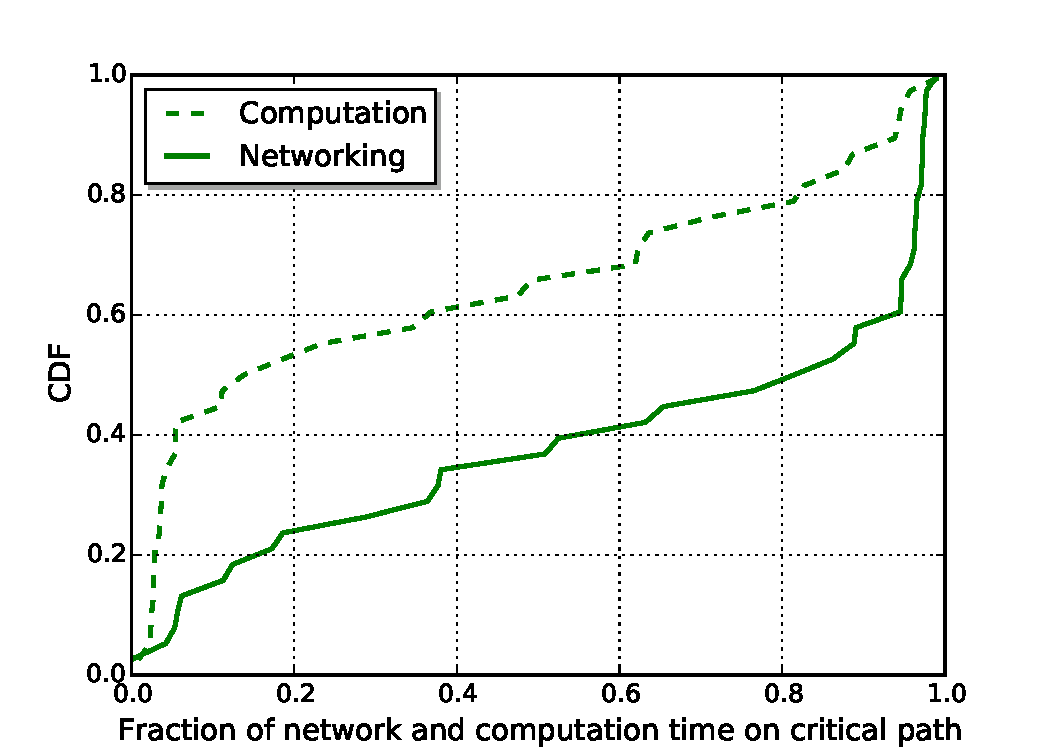
\includegraphics[width=1\linewidth]{./figures/computation/poor/desktop-b5-d150.pdf}
        \caption{Desktop browser, Poor lab\_4G}
        \label{fig:non-mobile-b5-d150}
    \end{subfigure}
   \begin{subfigure}{0.48\textwidth}
        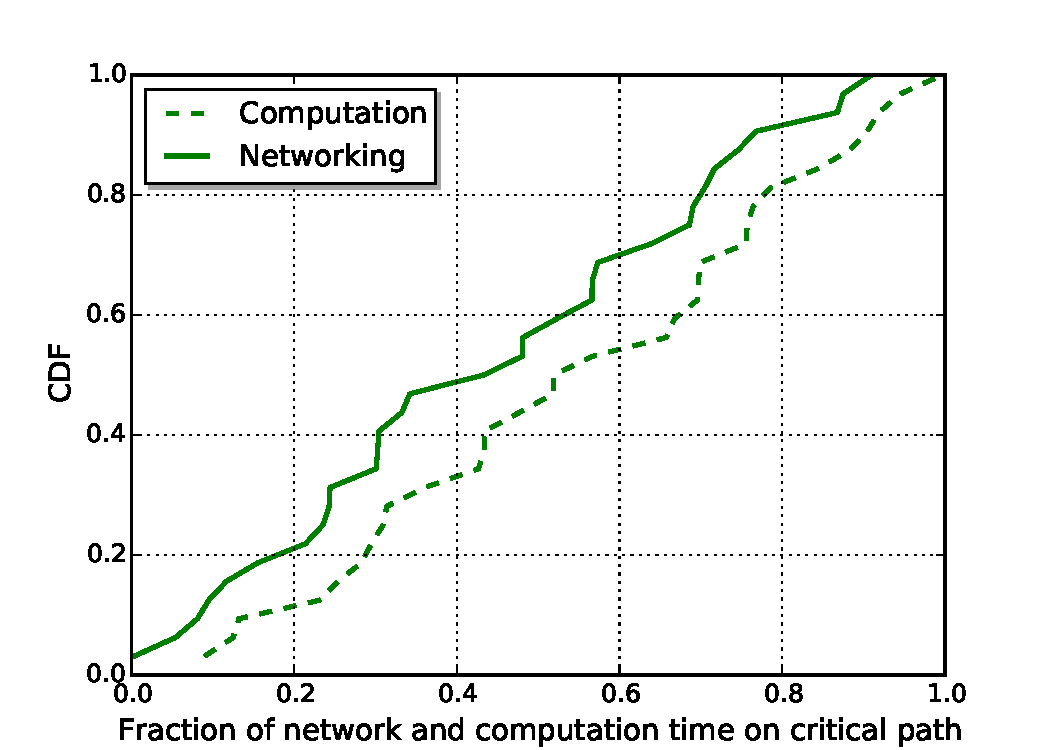
\includegraphics[width=1\linewidth]{./figures/computation/poor/mobile-b20-d150.pdf}
        \caption{Mobile browser, Poor lab\_Wifi}
        \label{fig:mobile-b20-d150}
    \end{subfigure}%
    \begin{subfigure}{0.48\textwidth}
    \centering
        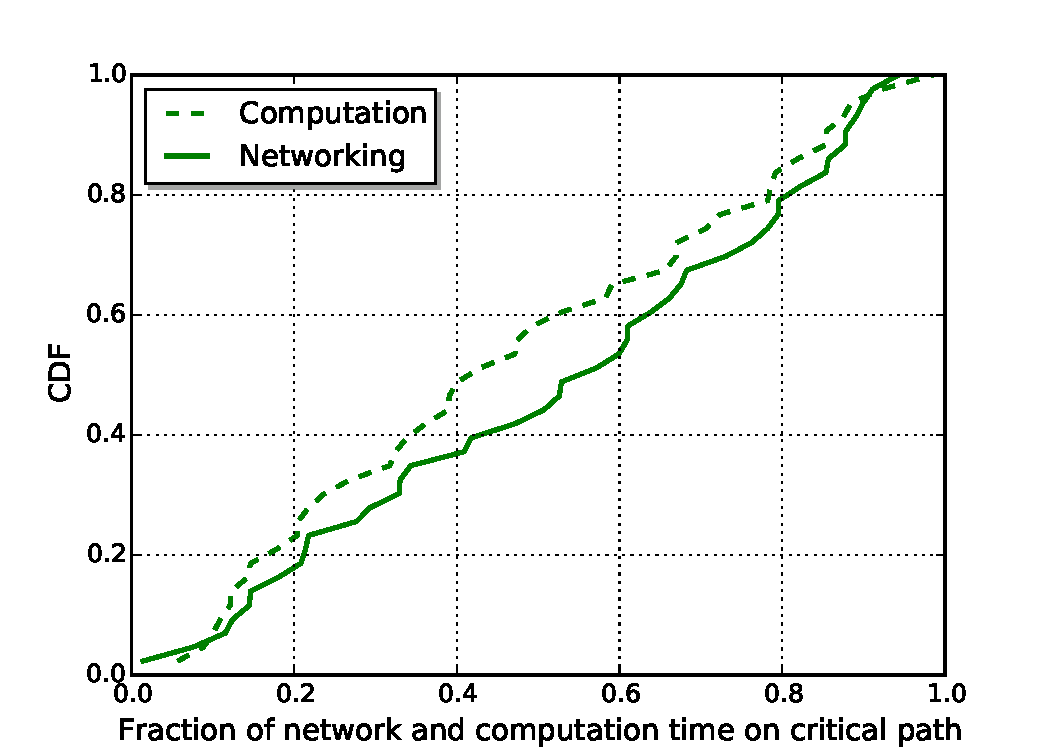
\includegraphics[width=1\linewidth]{./figures/computation/poor/mobile-b5-d150.pdf}
        \caption{Mobile browser, Poor lab\_4G}
        \label{fig:mobile-b5-d150}
    \end{subfigure}
      \caption{Poor Wireless Connectivity: Fraction of network and computation time on critical path. Even under poor network connectivity, computation is the bottleneck for mobile browsers. In contrast, under poor connectivity, network becomes even more of a bottleneck for desktop browsers.}
    \label{fig:comp_net_fraction_poor}
   \end{figure}


\subsection{Bottleneck when loading mpages}
Figure~\ref{fig:comp_network_mpage} shows that when loading {\em mpages} on the mobile browsers, computation is once again the bottleneck. In the median case, more than 60\% of the critical path is spent on computational activities in the median case.
\begin{figure}[!htb]
\centering{
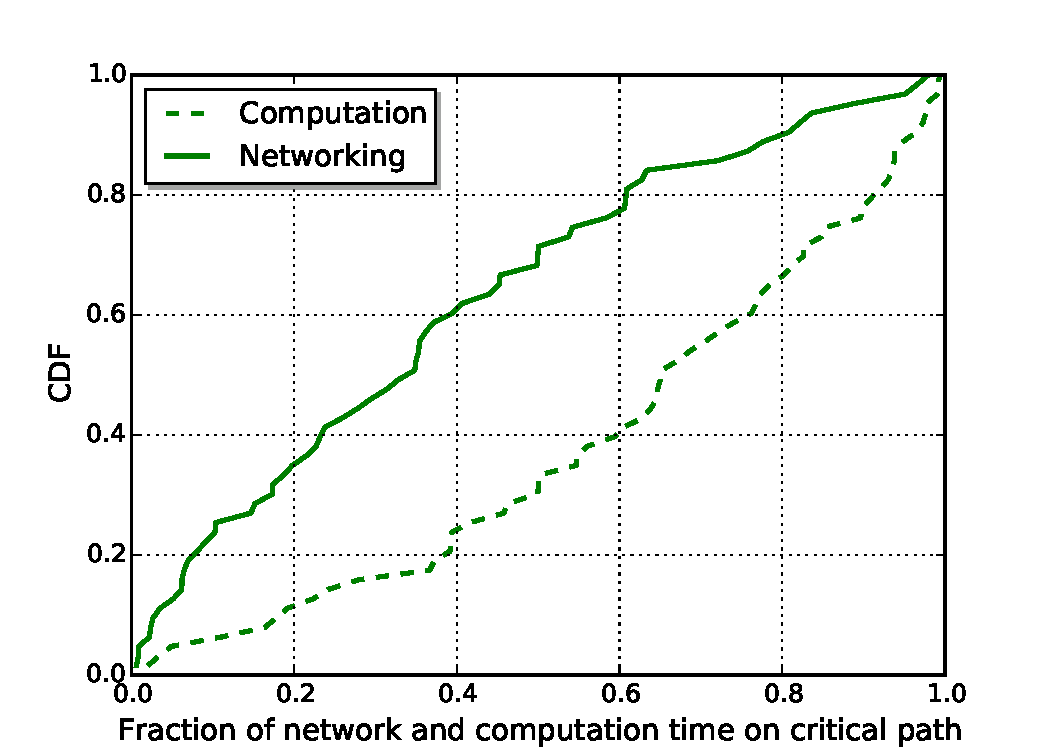
\includegraphics[scale=0.5]{./figures/computation/mobileversion_wifi_b20_d50.pdf}
\caption{Loading {\em mpages} on lab\_Wifi: The fraction of network and computation on critical path. }
\label{fig:comp_network_mpage}
}
\end{figure}


\subsection{Experiments on Samsung Galaxy S6}
 We ran the controlled page load experiments again on Samsung Galaxy S6, which has a 2100MHz CPU and octo-core, compared to the quad-core, 1700MHz Samsung S4 phones. Figure~\ref{fig:plt_s6_b5_d50} shows that the page load time on S6 is not much different compared to the page load time on S4. 

\noindent Interestingly, Figure~\ref{fig:comp-net-s6-b5-d50} shows that the computation is still a bottleneck for the page load, even under a better CPU specification. This results suggests that browsers are not utilizing the additional CPU capacity in newer phones effectively. 

\subsection{Experiments "in-the-wild"}
\label{sec:unrestricted}

\begin{figure}[!htb]
  \begin{subfigure}{0.48\textwidth}
     \centering{
        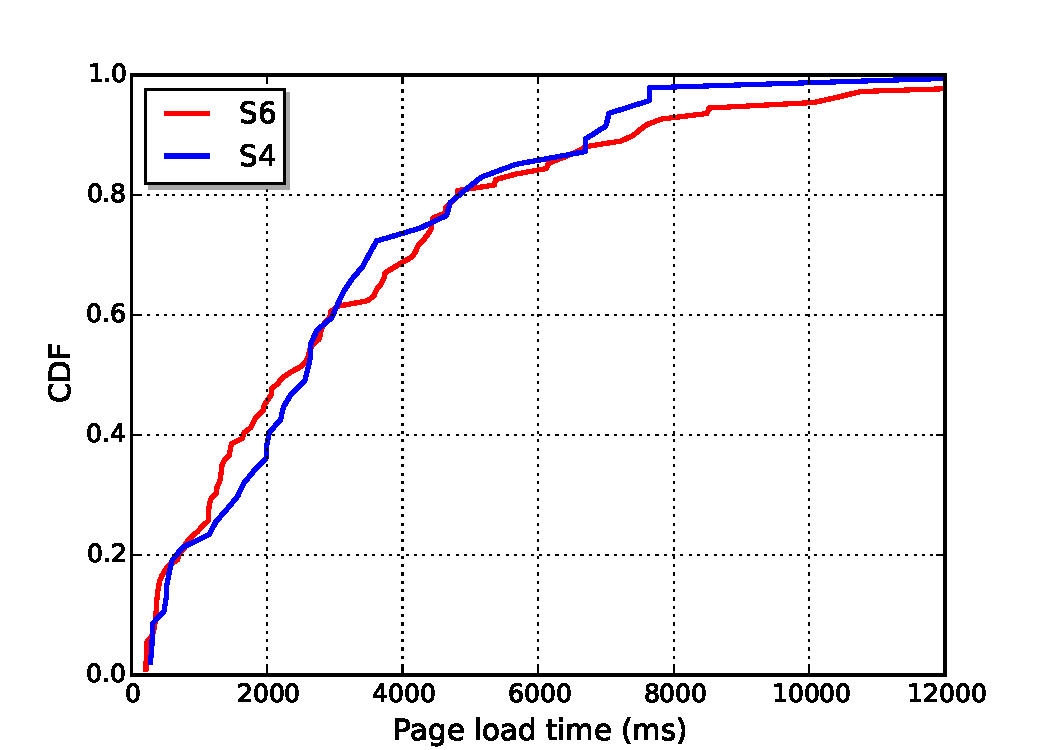
\includegraphics[width=1\linewidth]{./figures/s6/plt_s4_s6_mobile_b5_d50.pdf}
        \caption{PLTs when loading web pages on Samsung Galaxy S4 and S6 phones. The pages were loaded in the average lab\_4G network. }
        \label{fig:plt_s6_b5_d50}
    }
 \end{subfigure} \hspace{0.1in}%
\begin{subfigure}{0.48\textwidth}
            \centering{
        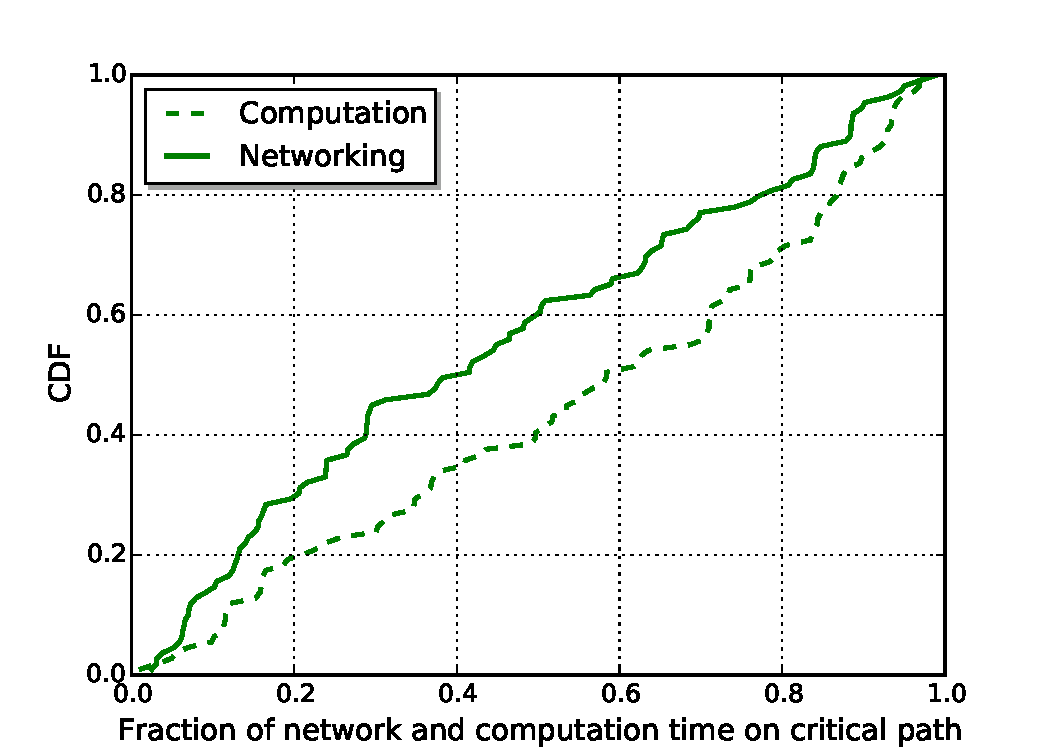
\includegraphics[width=1\linewidth]{./figures/s6/mobile_s6_b5-d50.pdf}
        \caption{Computation vs Networking on critical path  when loading pages in Samsung Galaxy S6 phones under average lab\_4G network conditions.}
        \label{fig:comp-net-s6-b5-d50}
        }
        \end{subfigure}
        \caption{Results from experiments on Samsung Galaxy S6}
        \label{fig:s6}
  \end{figure}


\noindent Finally, we load web pages on desktop and mobile browsers outside of our experimental testbed.  The web pages are fetched from the original Web server. The desktop browser uses the campus Ethernet connection (bandwidth 250Mbps), while the mobile browser uses the campus WiFi connection (bandwidth 30Mbps). The goal of this experiment is to study if the observations we make in the controlled setting also hold true in general. Note that as there are variances in networking parameters when running experiments {\em in-the-wild}, we cannot make generalizations in this case.

\begin{figure}[!htb]
\begin{minipage}[b]{.48\textwidth}
  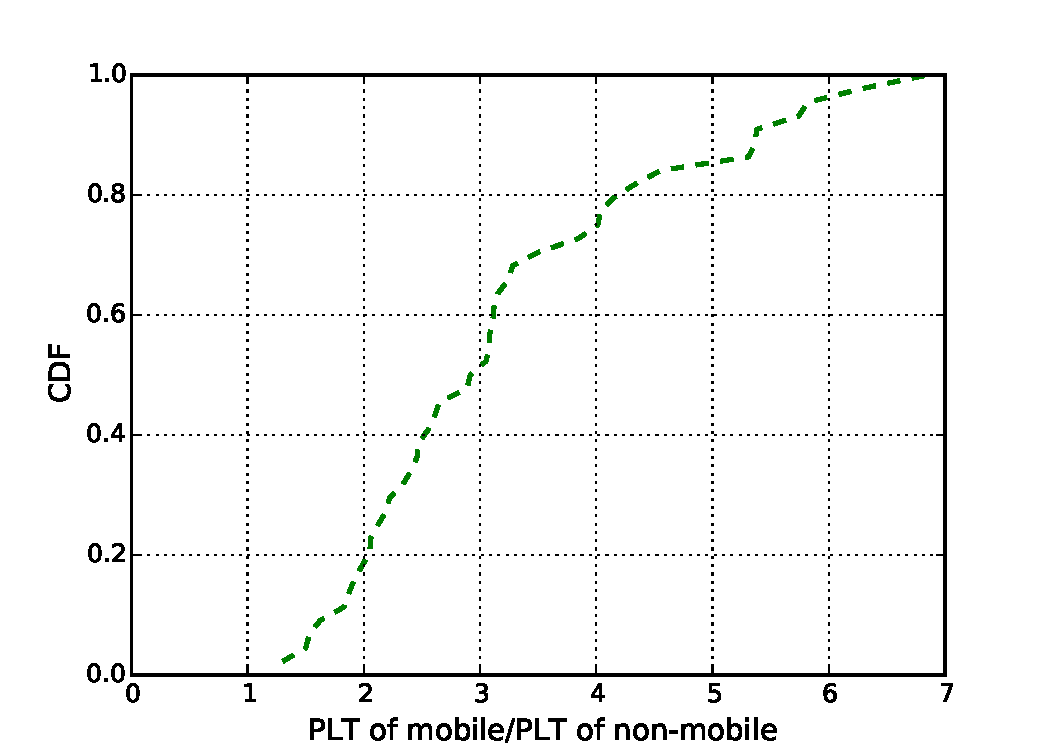
\includegraphics[width=\linewidth]{./figures/uncontrolled/mobile_desktop_plt_ratio_uncontrolled.pdf}
  \captionof{figure}{PLT difference between loading pages on mobile and desktop in-the-wild.}
  \label{fig:plt_uncontrolled_mobile_desktop}
\end{minipage}%
\hspace{0.5cm}
\begin{minipage}[b]{.48\textwidth}
  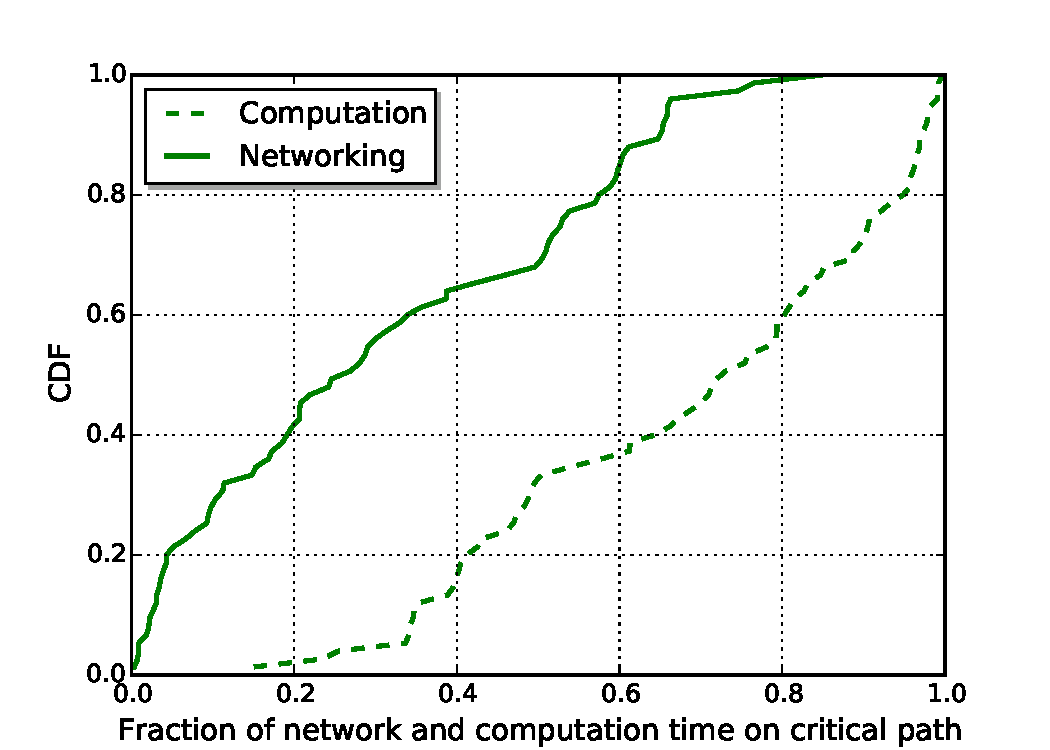
\includegraphics[width=\linewidth]{./figures/uncontrolled/mobile_uncontrolled.pdf}
  \captionof{figure}{Mobile browser in the wild: computation vs networking on critical path.}
  \label{fig:network_comp_uncontrolled_mobile}
\end{minipage}
\end{figure}

\noindent Figure~\ref{fig:plt_uncontrolled_mobile_desktop} shows the ratio of the time to load the page on mobile browsers and desktop browsers. The difference in page load time is even higher compared to the experiment in the controlled setting (Figure~\ref{fig:plt_desktop_mobile_mpage}). Loading pages on the mobile browser is three times as slow as the desktop in the median case. This is largely because of the difference in network speeds between Ethernet and WiFi.

\noindent Surprisingly, Figure~\ref{fig:network_comp_uncontrolled_mobile} shows that, similar to the controlled setting, the bottleneck in mobile browser remains computation.
%
%critical path analysis
%
\section{Critical path analysis}

Next, we study critical path in loading Web pages on mobile and desktop browsers. Summary of our observations are as follows:
\begin{itemize} 

\item Although number of Javascripts, CSS, images, and HTML evaluations seems to be similar on critical path, when the same web pages are loaded on the same network profiles, but objects are not exactly the same. In other words, activity type distribution remains similar, while they are different activities.

\item Each computation activity on the critical path, takes 4 times longer when is run on mobile browser compared to the desktop browser.

\end{itemize}
\subsection{Object downloads}

Figure~\ref{fig:numbytesall} depicts the total number of bytes downloaded when loading the original page and loading the {\em mpage} on a mobile browser in all network profiles. Even though {\em mpages} are designed to be smaller, we find that for 60\% of the pages, the total data downloaded remains the same. But for 30\% of the pages, the difference in size is over 60\%. The results suggests that {\em mpages} significantly reduce the size of a small number of pages, but for a large fraction of pages, there is not much difference between {\em mpages} and the original page.

Figure~\ref{fig:numbytescp} shows the bytes downloaded on the critical path for original page and {\em mpage}. Recall that only objects loaded in the critical path contribute to the page load time; other objects are loaded in parallel. Here we find that {\em mpages} reduce the number of objects loaded in the critical path for over 40\% of the pages. In other words, {\em mpages} does reduce the network latency on the critical path.

However, the page load time does not reduce significantly when loading {\em mpages} compared to the original pages (see Figure~\ref{fig:plt_desktop_mobile_mpage}). This is because the computation is the bottleneck when loading {\em mpages} on the mobile browser, as shown in Figure~\ref{fig:comp_network_mpage}. In a separate experiment (not shown here), we find that loading {\em mpages} does not reduce the computation time on the critical path. In fact, the computation time is slightly worse. 

\subsection{Similarity metric}

We load the same pages on mobile and desktop browsers, under the same network environments. This lets us compare the critical path of the page load on mobile and desktop browsers. The critical path consists of a series of activities such as loading an object, evaluating a Javascript, etc. In addition, each activity is associated with a unique URL corresponding to the activity. For example, the URL of the object to be loaded, or the URL of the Javascript to be evaluated.


\begin{figure}[!htb]
\begin{minipage}[b]{.48\textwidth}
  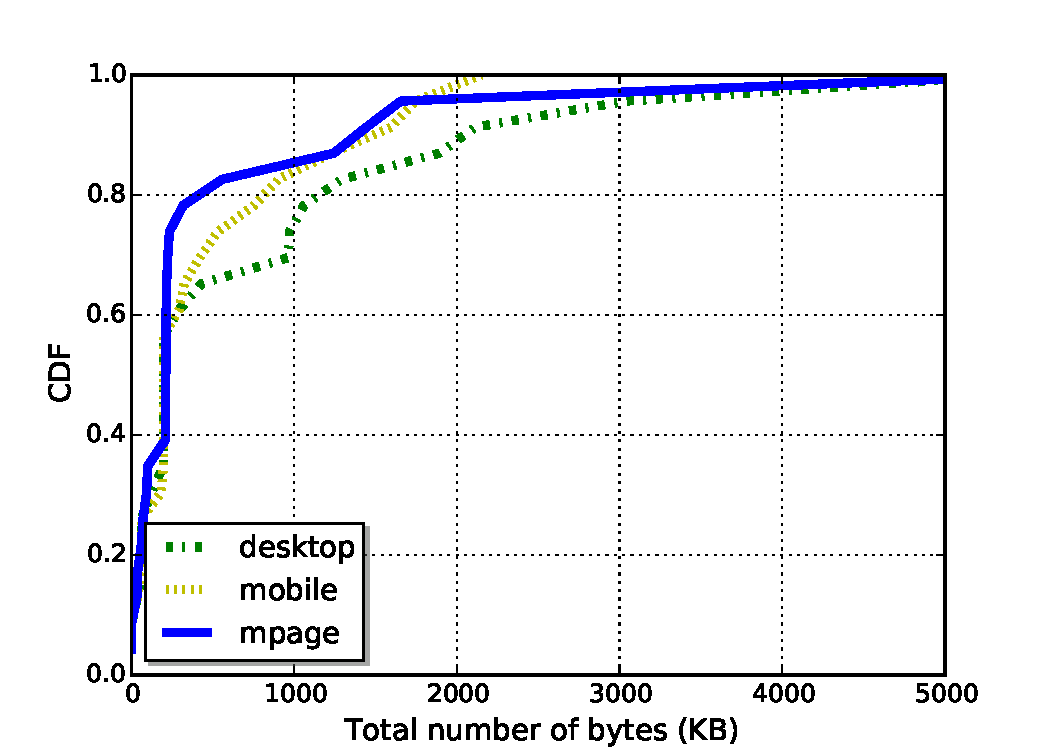
\includegraphics[width=\linewidth]{./figures/criticalpath/num_bytes_all.pdf}
  \captionof{figure}{Number of total bytes downloaded for{ \em mobile} and{ \em mpage} }
  \label{fig:numbytesall}
\end{minipage}%
\hspace{0.5cm}
\begin{minipage}[b]{.48\textwidth}
  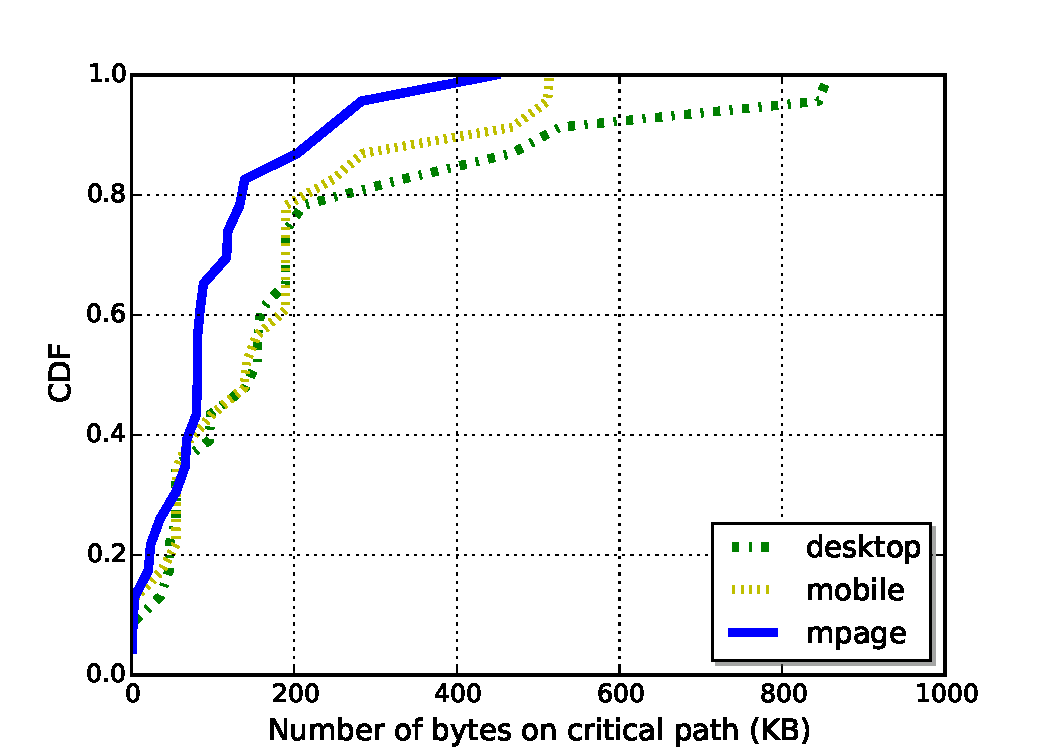
\includegraphics[width=\linewidth]{./figures/criticalpath/num_bytes_cp.pdf}
  \captionof{figure}{Number of bytes download on critical path for{ \em mobile} and{ \em mpage}}
  \label{fig:numbytescp}
\end{minipage}
\end{figure}

\noindent We define similarity metric as follows: the fraction of time the same <URL, activity> pair occurs  both on the critical path of the mobile page load and the critical path of the desktop page load. If the number of elements on the critical path are not equal, we pad the smaller critical path with null activities.

\noindent Figure~\ref{fig:similarity} shows the similarity metric across all network profiles. Even when the same page is being loaded under the same network profile, the critical path is identical only for 20\% of pages. For another 20\% of the pages, only 50\% of the critical path is similar. This result has big implications for optimization. It shows that optimizing a specific object, such as making a specific Javascript object smaller, may not have the same effect on mobile browsers as they would desktop browsers.

\begin{figure}[!htb]
  \centering
    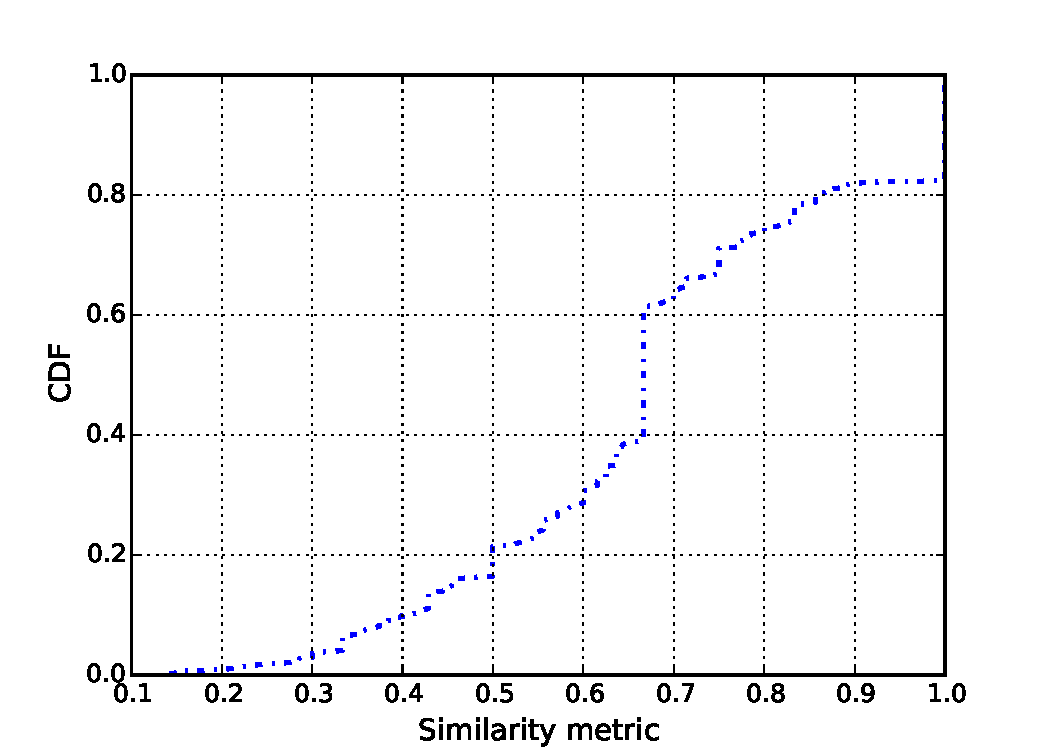
\includegraphics[width=0.5 \textwidth]{./figures/criticalpath/similarity.pdf}
  \caption{Similarity metric: the fraction of time the same <URL, activity> pair occur on the critical path of both mobile and desktop page load. }
  \label{fig:similarity}
\end{figure}

\noindent Next, we relax the definition of similarity and look at the percentage of time the same activity occur on the critical paths. For example, if there two Javascript activities on both critical paths, but the URLs corresponding to the Javascript are different, we still define the two activities as being similar.  For this definition of similarity, we also include the experiments where we loaded the mobile version of the pages.

\noindent Figure \ref{fig:bar_plot_percentage} shows the percentage of each activity on the critical path across all pages and network profiles. In terms of the activities, we see that the critical path is very similar. In other words, for every page, the activities on the critical path in terms of Javascript evaluation, HTML parsing etc are similar on desktop and mobile browsers. But the critical paths differ in terms of, for example, which Javascript is being evaluated. One of the implications of this result is that, optimizations that target a class of activities, such as reducing the time to download all Javascript objects, are likely to provide benefits across mobile and desktop browsers.

\begin{figure}[!htb]
  \centering
    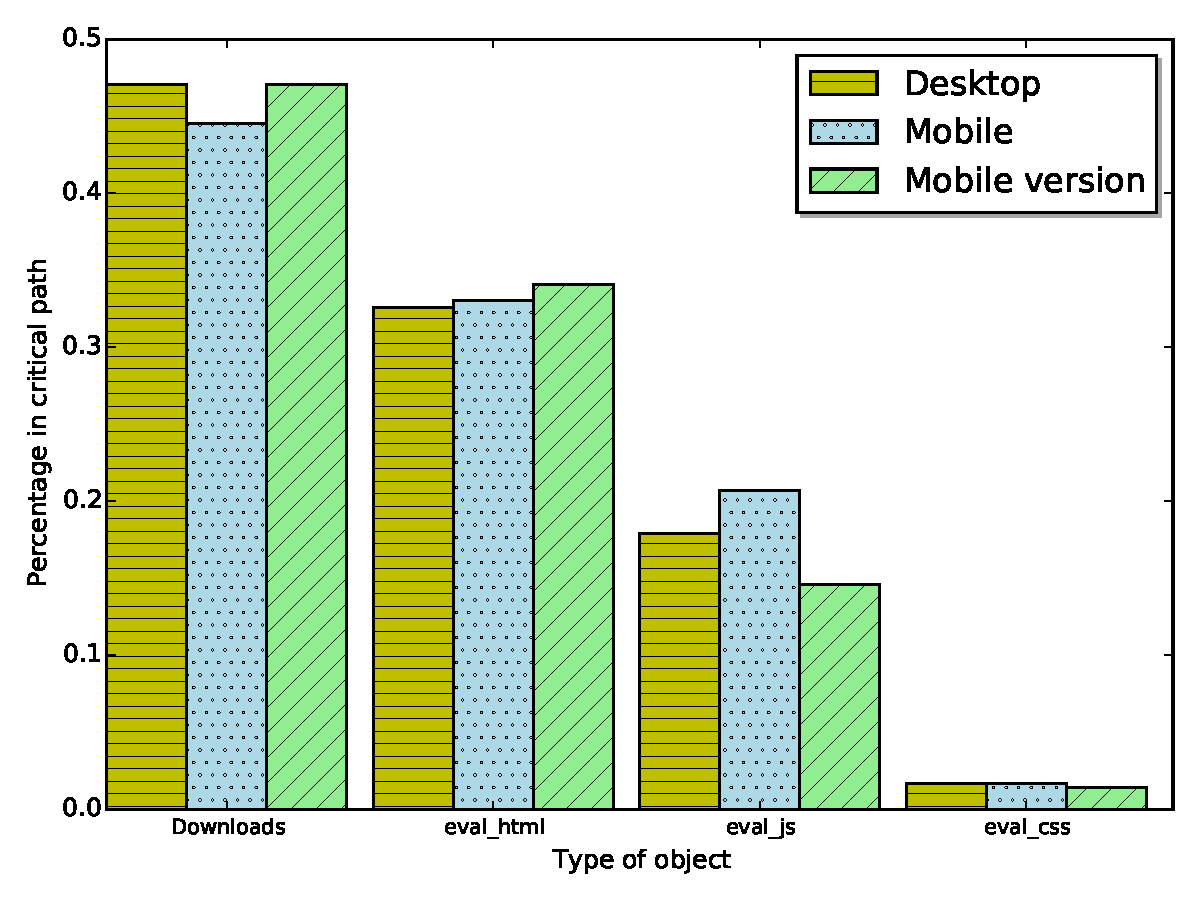
\includegraphics[width=0.5\textwidth]{./figures/criticalpath/bar_plot_percentage.pdf}
  \caption{Fraction of different activities on the critical path. }
  \label{fig:bar_plot_percentage}
\end{figure}

\subsection{Latency for each activity on the critical path}

Finally, we measure the difference in latencies when performing the same activity on the mobile versus the desktop browser.  To this end, we identify each activity on the critical path of either the desktop load or the mobile load. We then compare the latency of this activity when loading on the desktop versus loading on the mobile browser. Since we load the exact same page, an activity such as loading a specific Javascript  will have to be performed both on the desktop load and the mobile load.

\noindent Figure~\ref{fig:bar_plot_percentage} shows the time take of each activity to be performed on the mobile versus the desktop browser. Each computation activity takes over 4 times longer to perform on the mobile browser versus the desktop browser. This is the core reason for the computational bottleneck on mobile browsers. For 50\% of the web pages, it takes slightly longer to perform network activities on the mobile browser compared to desktop browser. This can possibly be because of a less optimized network stack on the mobile browser compared to desktop browser.

\begin{figure}[!htb]
  \centering
    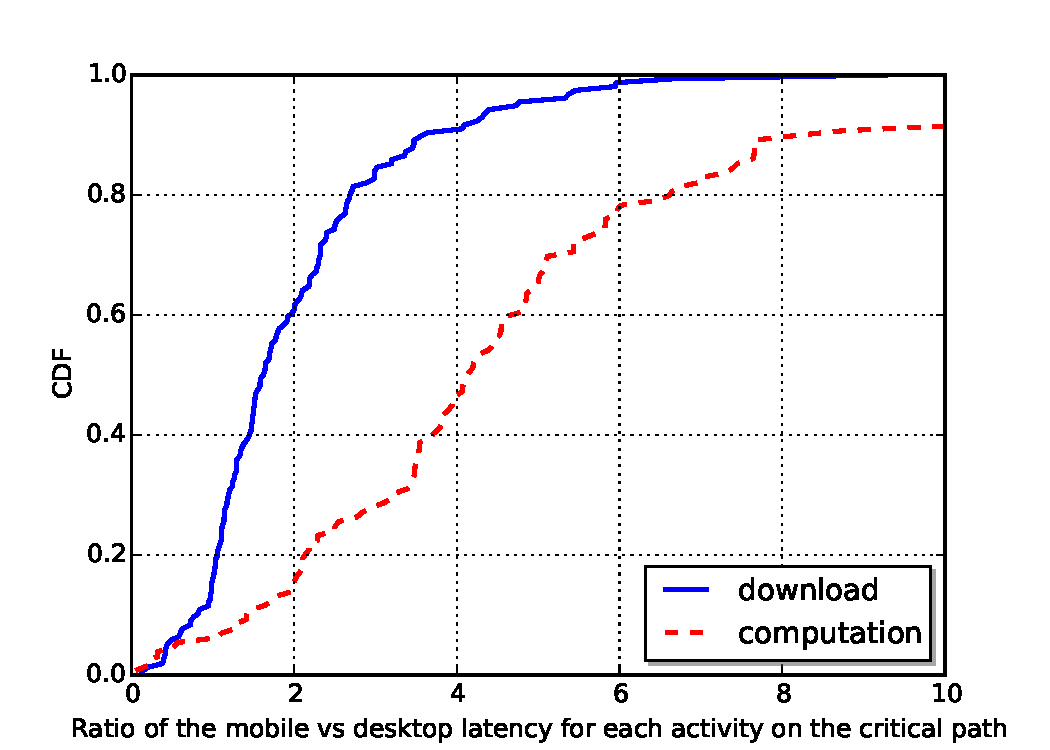
\includegraphics[width=0.5\textwidth]{./figures/criticalpath/latency_comp_network_b20-d50.pdf}
  \caption{Time taken for each activity on the critical path to be performed on the mobile versus desktop browser. Results from loading pages on average lab\_Wifi network. }
  \label{fig:bar_plot_percentage}
\end{figure}





%!TEX root = ../main.tex
\chapter{Page optimization}\label{ch:optimization}
In pursuing our goal to improve page load time so far, we have characterized the main bottleneck in a page load process on mobile devices. Our next step is to study the effect of optimizations on the page load time. There has been several industry tools that also study the page and suggest optimizations.
Google PageSpeed Insights \cite{pagespeedinsight} and Yahoo's YSlow \cite{yslow} are two noteable current web optimization platform. Although they both are trying to suggest optimizations to improve the overall web site's performance, but they suffer from some major problems.
Two main issues with Google PageSpeed Insights and Yahoo's YSlow solutions are as follows:
 \begin{itemize}
  \item They do not directly measure the benefit of an optimization on the page load time. Instead, they use a scoring mechanism that do not necessarily correlate well with the real page load improvements.
  \item They are using fixed set of rules and do not consider optimizing for each particular case.\\
   
\noindent For example, PageSpeed Insights encourages users to inline (small) scripts in the HTML source file to avoid additional roundtrip times.
On the contrary,  YSlow recommends to make Javascript and CSS scripts external, to benefit from possible caching. This differences arise because of not considering the varying nature of servers, clients and network connections.\\
\noindent We should also note that modification do not always help.
For example, a popular improvement to reduce the download time is enabling compression in server side. Modern browsers support this feature automatically and decompress the received objects. Although this technique seems to be always beneficial, one should be careful about the gain achieved in reducing download time against increased computing time needed to decompress the whole session.
\end{itemize}

\noindent In this chapter, first, we study current web page optimization solutions, mainly Google's PageSpeed Insights and Yahoo's YSlow . Then we analyze these optimizations and study their effect on page load time using our testbed.

\noindent We then, illustrate building blocks of our future platform which scores each optimization based on it's contribution to the page load time. Having a platform that shows the effects of optimizations on page load time and considers the dynamic nature of servers, clients and network connections at the same time, would enable us to more precisely suggest customized optimizations for each particular case.
\section{Current page optimization solutions}
\subsection{Google's PageSpeed Insights}
PageSpeed Insights \cite{pagespeedinsight} is a tool that helps developers optimize their web pages by analyzing the pages and generating tailored suggestions to make the pages faster.
PageSpeed Insights measures the performance of a page for mobile devices and desktop devices. It fetches the URL twice, once with a mobile user-agent, and once with a desktop-user agent. PageSpeed Insights analysis does not use real devices. It fetches a site with a webkit renderer (the same rendering engine that powers Chrome and Safari) that emulates both mobile device and desktop devices.\\

\noindent The PageSpeed Score ranges from 0 to 100 points. The higher the score, the better the performance. However, since the performance of a network connection varies considerably, PageSpeed Insights only considers the network-independent aspects of page performance: the server configuration, the HTML structure of a page, and its use of external resources such as images, JavaScript, and CSS. Implementing the suggestions should improve the relative performance of the page. However, the absolute performance of the page will still be dependent upon a user's network connection.\\\\

\subsubsection{Architecture:}
Developer makes a simple HTTP request to google PageSpeed Insights servers and gives a URL to fetch. PageSpeed Insights will fetch and render that URL, then runs the Page Speed library on it and gives back the result as depicted in figure \ref{fig:pagespeed}
\begin{figure}[!htb]
\centering{
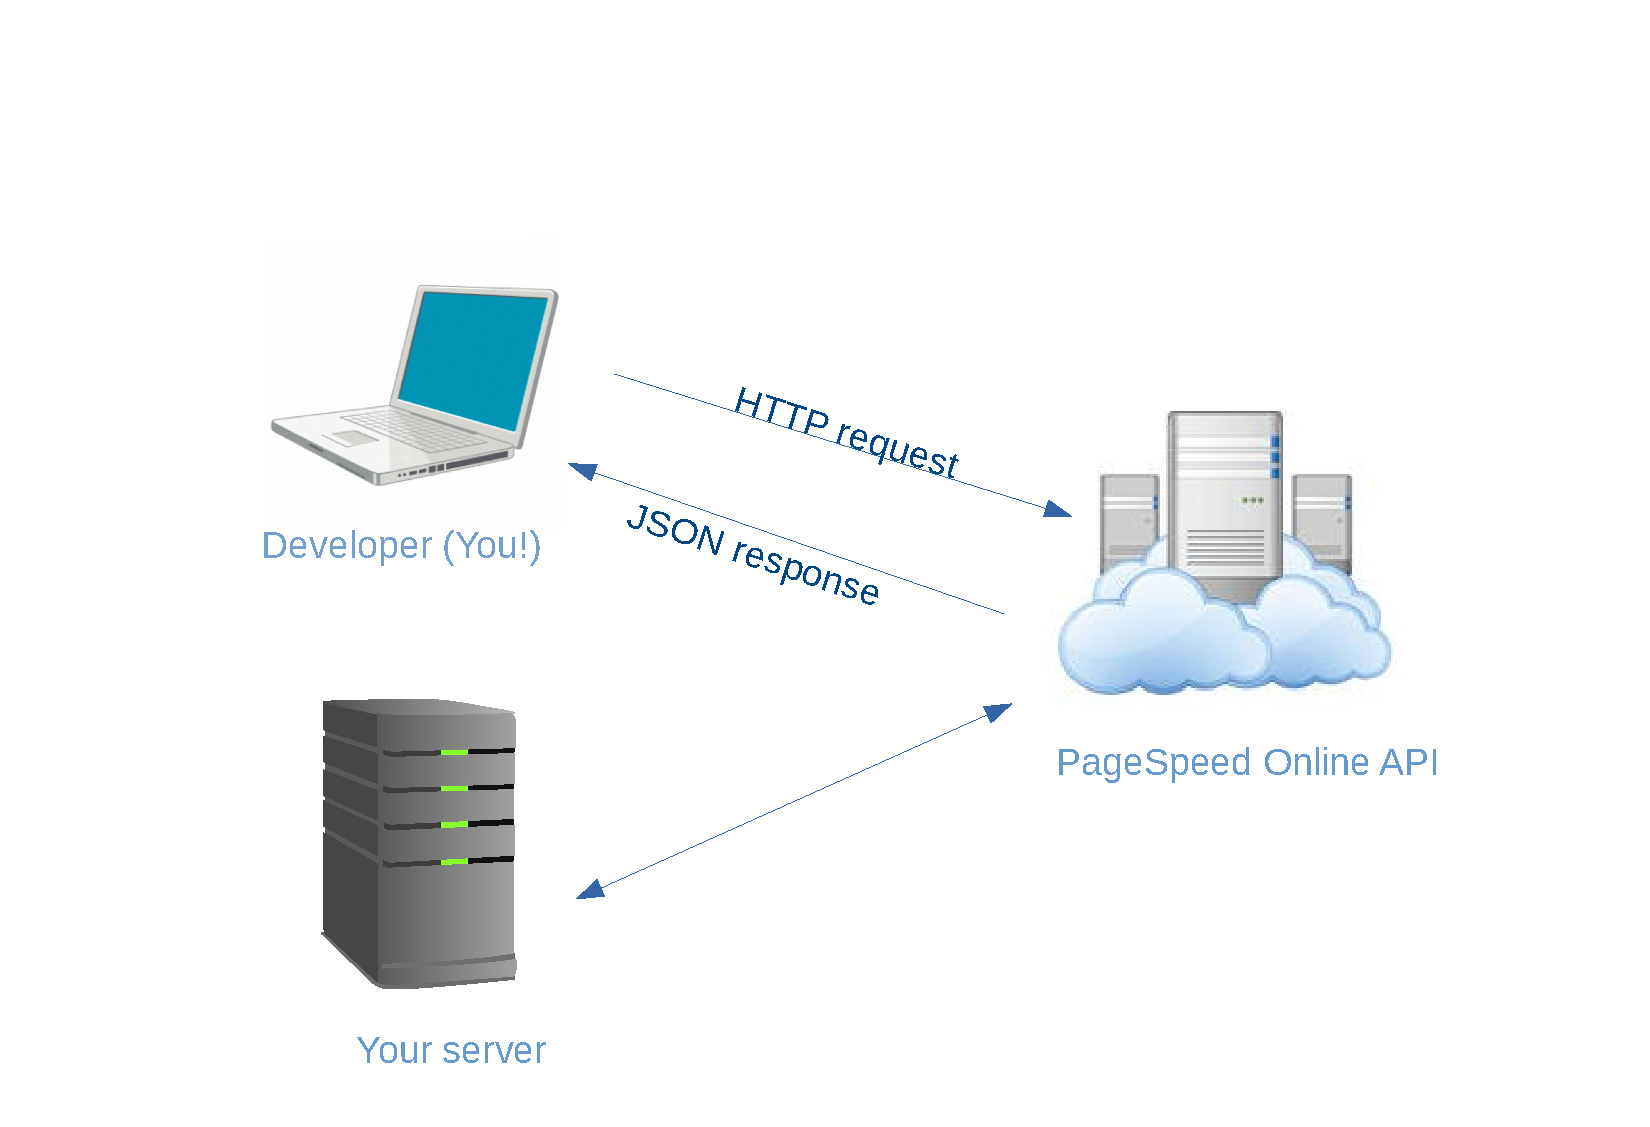
\includegraphics[scale=0.5]{./figures/optimization/pagespeed.pdf}
\caption{PageSpeed Insights online API}
\label{fig:pagespeed}
}
\end{figure}

\subsubsection {PageSpeed SDK}
A webpage is fetched and rendered using {\em pagespeed\_webkit} and then the defined rules  in {\em lib/trunk/src/pagespeed/rules} are applied and the formatted results are presented.\\
Results of all the rules are presented to the user. Each PageSpeed rule generates an impact number (an unbounded floating point value) that indicates the importance or priority of implementing the rule-result suggestions for the rule, relative to other rules.\\

\noindent For instance, if enabling compression would save 1MB, while optimizing images would save 500kB, the {\em "Enable Compression"} rule would have an impact value that is twice that of the {\em "Optimize Images"} rule. An impact of zero indicates that there is no suggestion for improvement for that rule.
Following is a code snippet of a sample response of PageSpeed Insights API:
\begin{minted}[frame=leftline, framerule=1.5pt, rulecolor=\color{blue}]{json}
{
 "kind": "pagespeedonline#result",
 "id": "/speed/pagespeed",
 "responseCode": 200,
 "title": "PageSpeed Home",
 "score": 90,
 "pageStats": {
  "numberResources": 22,
  "numberHosts": 7,
  "totalRequestBytes": "2761",
  "numberStaticResources": 16,
  "htmlResponseBytes": "91981",
  "cssResponseBytes": "37728",
  "imageResponseBytes": "13909",
  "javascriptResponseBytes": "247214",
  "otherResponseBytes": "8804",
  "numberJsResources": 6,
  "numberCssResources": 2
 },
   "comment": "..."
   "MinifyJavaScript": {
    "localizedRuleName": "Minify JavaScript",
    "ruleImpact": 0.1417,
   "comment": "..."
 }
}
\end{minted}
The improvements/fixes shown on PageSpeed Insights are sorted in decreasing order of their {\em "Rule Impact"} value. The one that has more Impact value will be shown first, which means that fixing it would have significant improvement in webpage performance.
\subsubsection{ Effect of PageSpeed Insights' rules on page load time}
Goal of these experiments is to see how much effect the suggestions of PageSpeed Insights has on page load time. For this purpose, we have considered 5 websites for which PageSpeed suggests to Inline JS/CSS, Minify HTML/CSS/JS and Optimize images. For each website, entire website is downloaded locally on testbed and modified to implement three suggestions; Inlining, minification and optimizing images separately to see the impact of each change on page load times. \\
\noindent We performed these experiments with three different network profiles b1-d50, b5-d50 and b20-d50 where "b" stands for bandwidth and "d" stands for delay. Results for b20-d5- are only shown here.

\begin{enumerate}
\item {\textbf {Inlining:}}\\
PageSpeed Insights suggests to inline only specific JS/CSS. Inlining should ideally help to reduce overall page load time, specifically total download time.
Experiments were done with 4 websites of which inlining actually helped two and didn't help other two as shown in figure \ref{fig:InsightsInlining_b20_d50} . For first two sites page load time did not improve; in fact, worsened.

\begin{figure}[!htb]
  \centering
    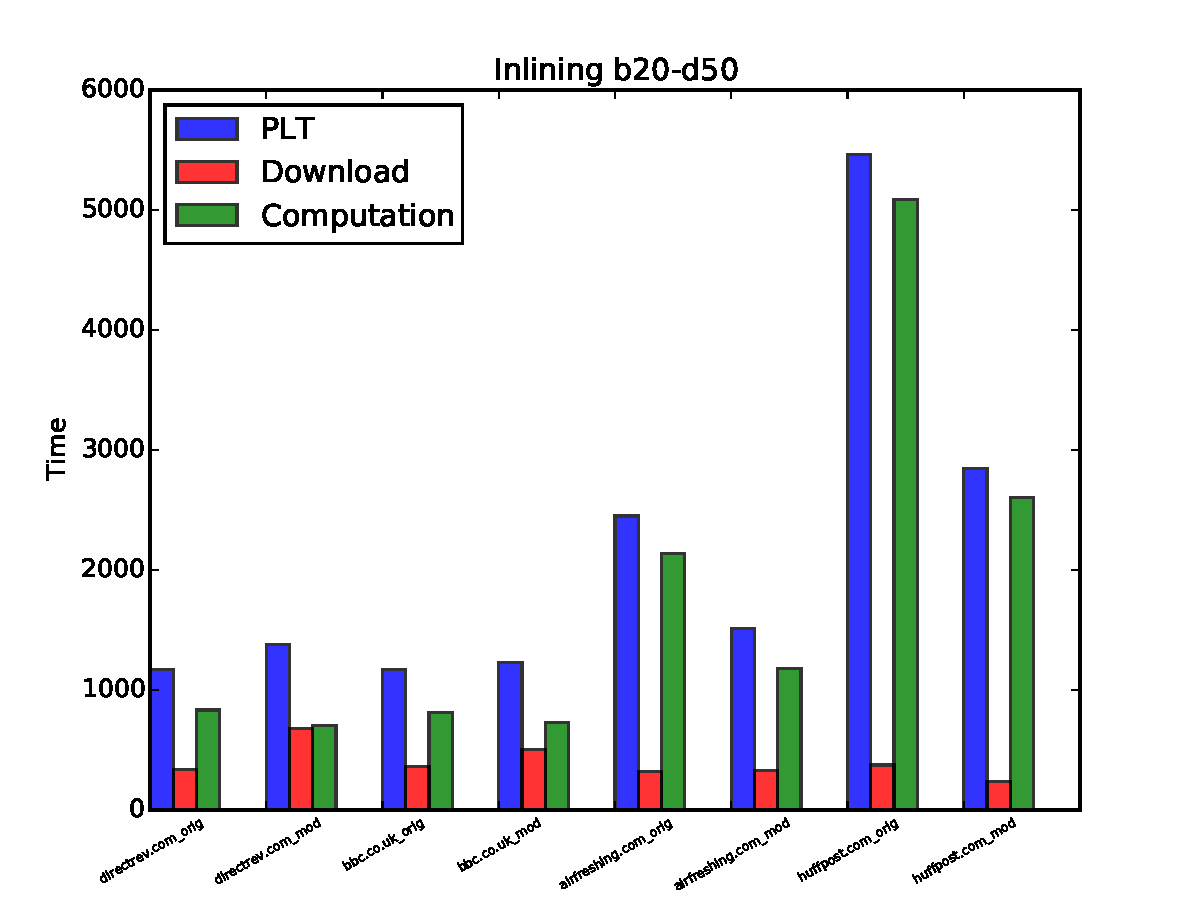
\includegraphics[width=0.85 \textwidth]{./figures/optimization/InsightsInlining_b20_d50.pdf}
  \caption {Page load time before/after inlining using PageSpeed insights }
  \label{fig:InsightsInlining_b20_d50}
\end{figure}

% add more explanation

\item  {\textbf {Optimize Images:}}\\
PageSpeed Insights suggests to optimize few images so that their size is reduced which should eventually help reducing page load time. One disadvantage to this suggestion is size reduction is at the cost of high quality. Compressing images results in low quality which can affect user experience.\\

As we observe from figure \ref{fig:InsightsOptimizeImages_b20_d50}, optimizing images, helps to reduce page load time for {\em huffpost.com} and {\em airfreshing.com} while does not help in {\em youku.com} and {\em directrev.com} and even hurts in {\em bbc.co.uk}.
\begin{figure}[!htb]
  \centering
    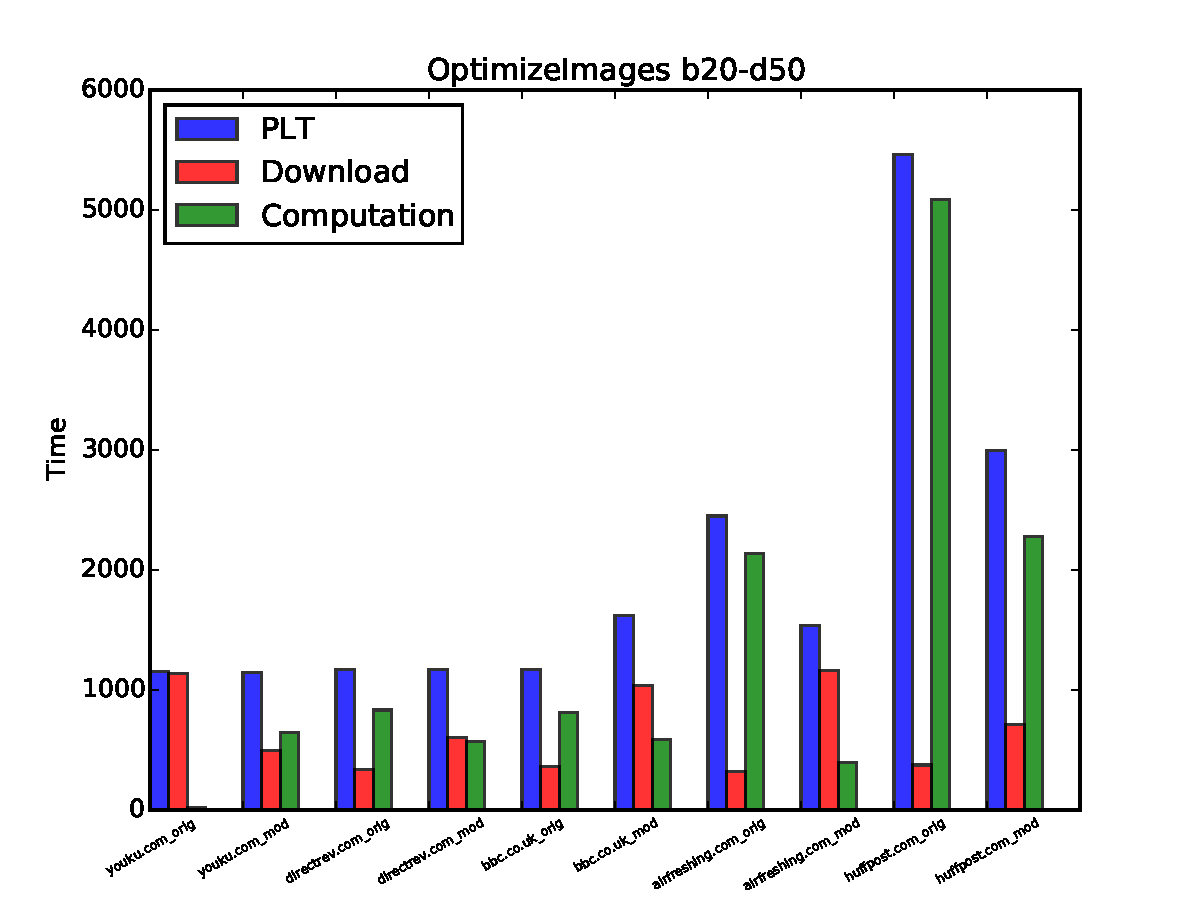
\includegraphics[width=0.85 \textwidth]{./figures/optimization/InsightsOptimizeImages_b20_d50.pdf}
  \caption {Page load time before/after optimizing images using PageSpeed insights }
  \label{fig:InsightsOptimizeImages_b20_d50}
\end{figure}

\item {\textbf{Minification:}}\\
Page speed Insights suggests to minfiy JS/CSS/HTML to reduce the size of those files so that download time is reduced and page load time is improved. As shown in figure  \ref{fig:InsightsOptimizeImages_b20_d50}, minifcation alone is not always helping to reduce page load time. We can see again, minification has helped {\em directrev.com }, {\em airfreshing.com} and {\em huffpost.com} but, hurt {\em youku.com} and {\em bbc.co.uk}.
\begin{figure}[!htb]
  \centering
    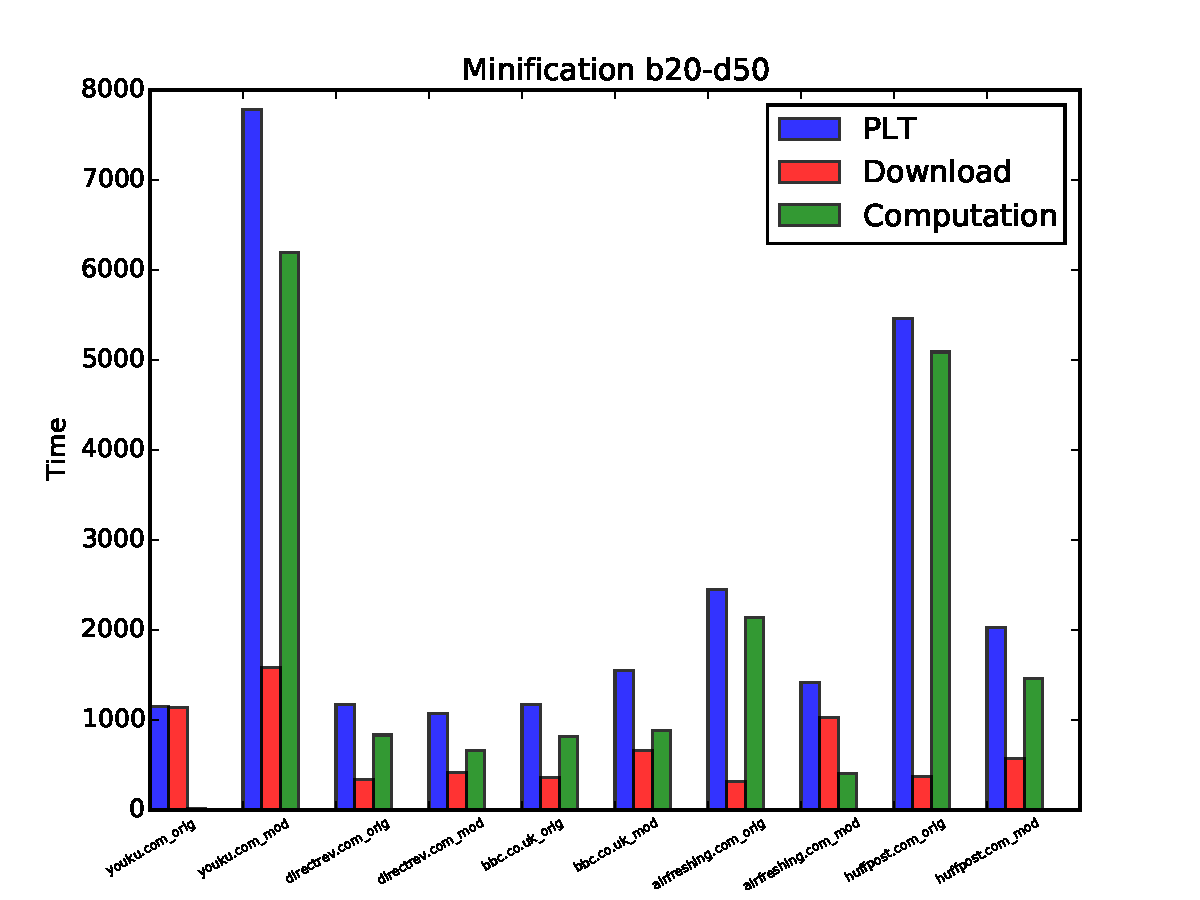
\includegraphics[width=0.85 \textwidth]{./figures/optimization/InsightsMinification_b20_d50.pdf}
  \caption {Page load time before/after Minification using PageSpeed insights }
  \label{fig:InsightsMinification_b20_d50}
\end{figure}

\end{enumerate}

\subsection{Yahoo's YSlow}
Yahoo's YSlow \cite{yslow}  grades web page based on one of three predefined ruleset or a user-defined ruleset.
It also offers suggestions for improving the page's performance and provides tools for performance analysis.\\

\noindent YSlow works in three phases to generate its results.

\begin{enumerate}

\item YSlow crawls the DOM to find all the components (images, scripts, stylesheets, etc.) in the page. After crawling the DOM, YSlow loops through Firebug's \cite{firebug} Net Panel components and adds those to the list of components already found in the DOM.
\item YSlow gets information about each component: size, whether it was gzipped, Expires header, etc. YSlow gets this information from Firebug's Net Panel if it's available. If the component's information is not available from Net Panel (for example, the component was read from cache or it had a 304 response), YSlow makes an XMLHttpRequest to fetch the component and track its headers and other necessary information.
\item YSlow takes all this data about the page and generates a grade for each rule, which produces the overall grade.
\end{enumerate}

\noindent Figure \ref{fig:yslow_stonybrook} shows a sample analysis for {\em www.cs.stonybrook.edu} using YSlow.
\begin{figure}[!htb]
  \centering
    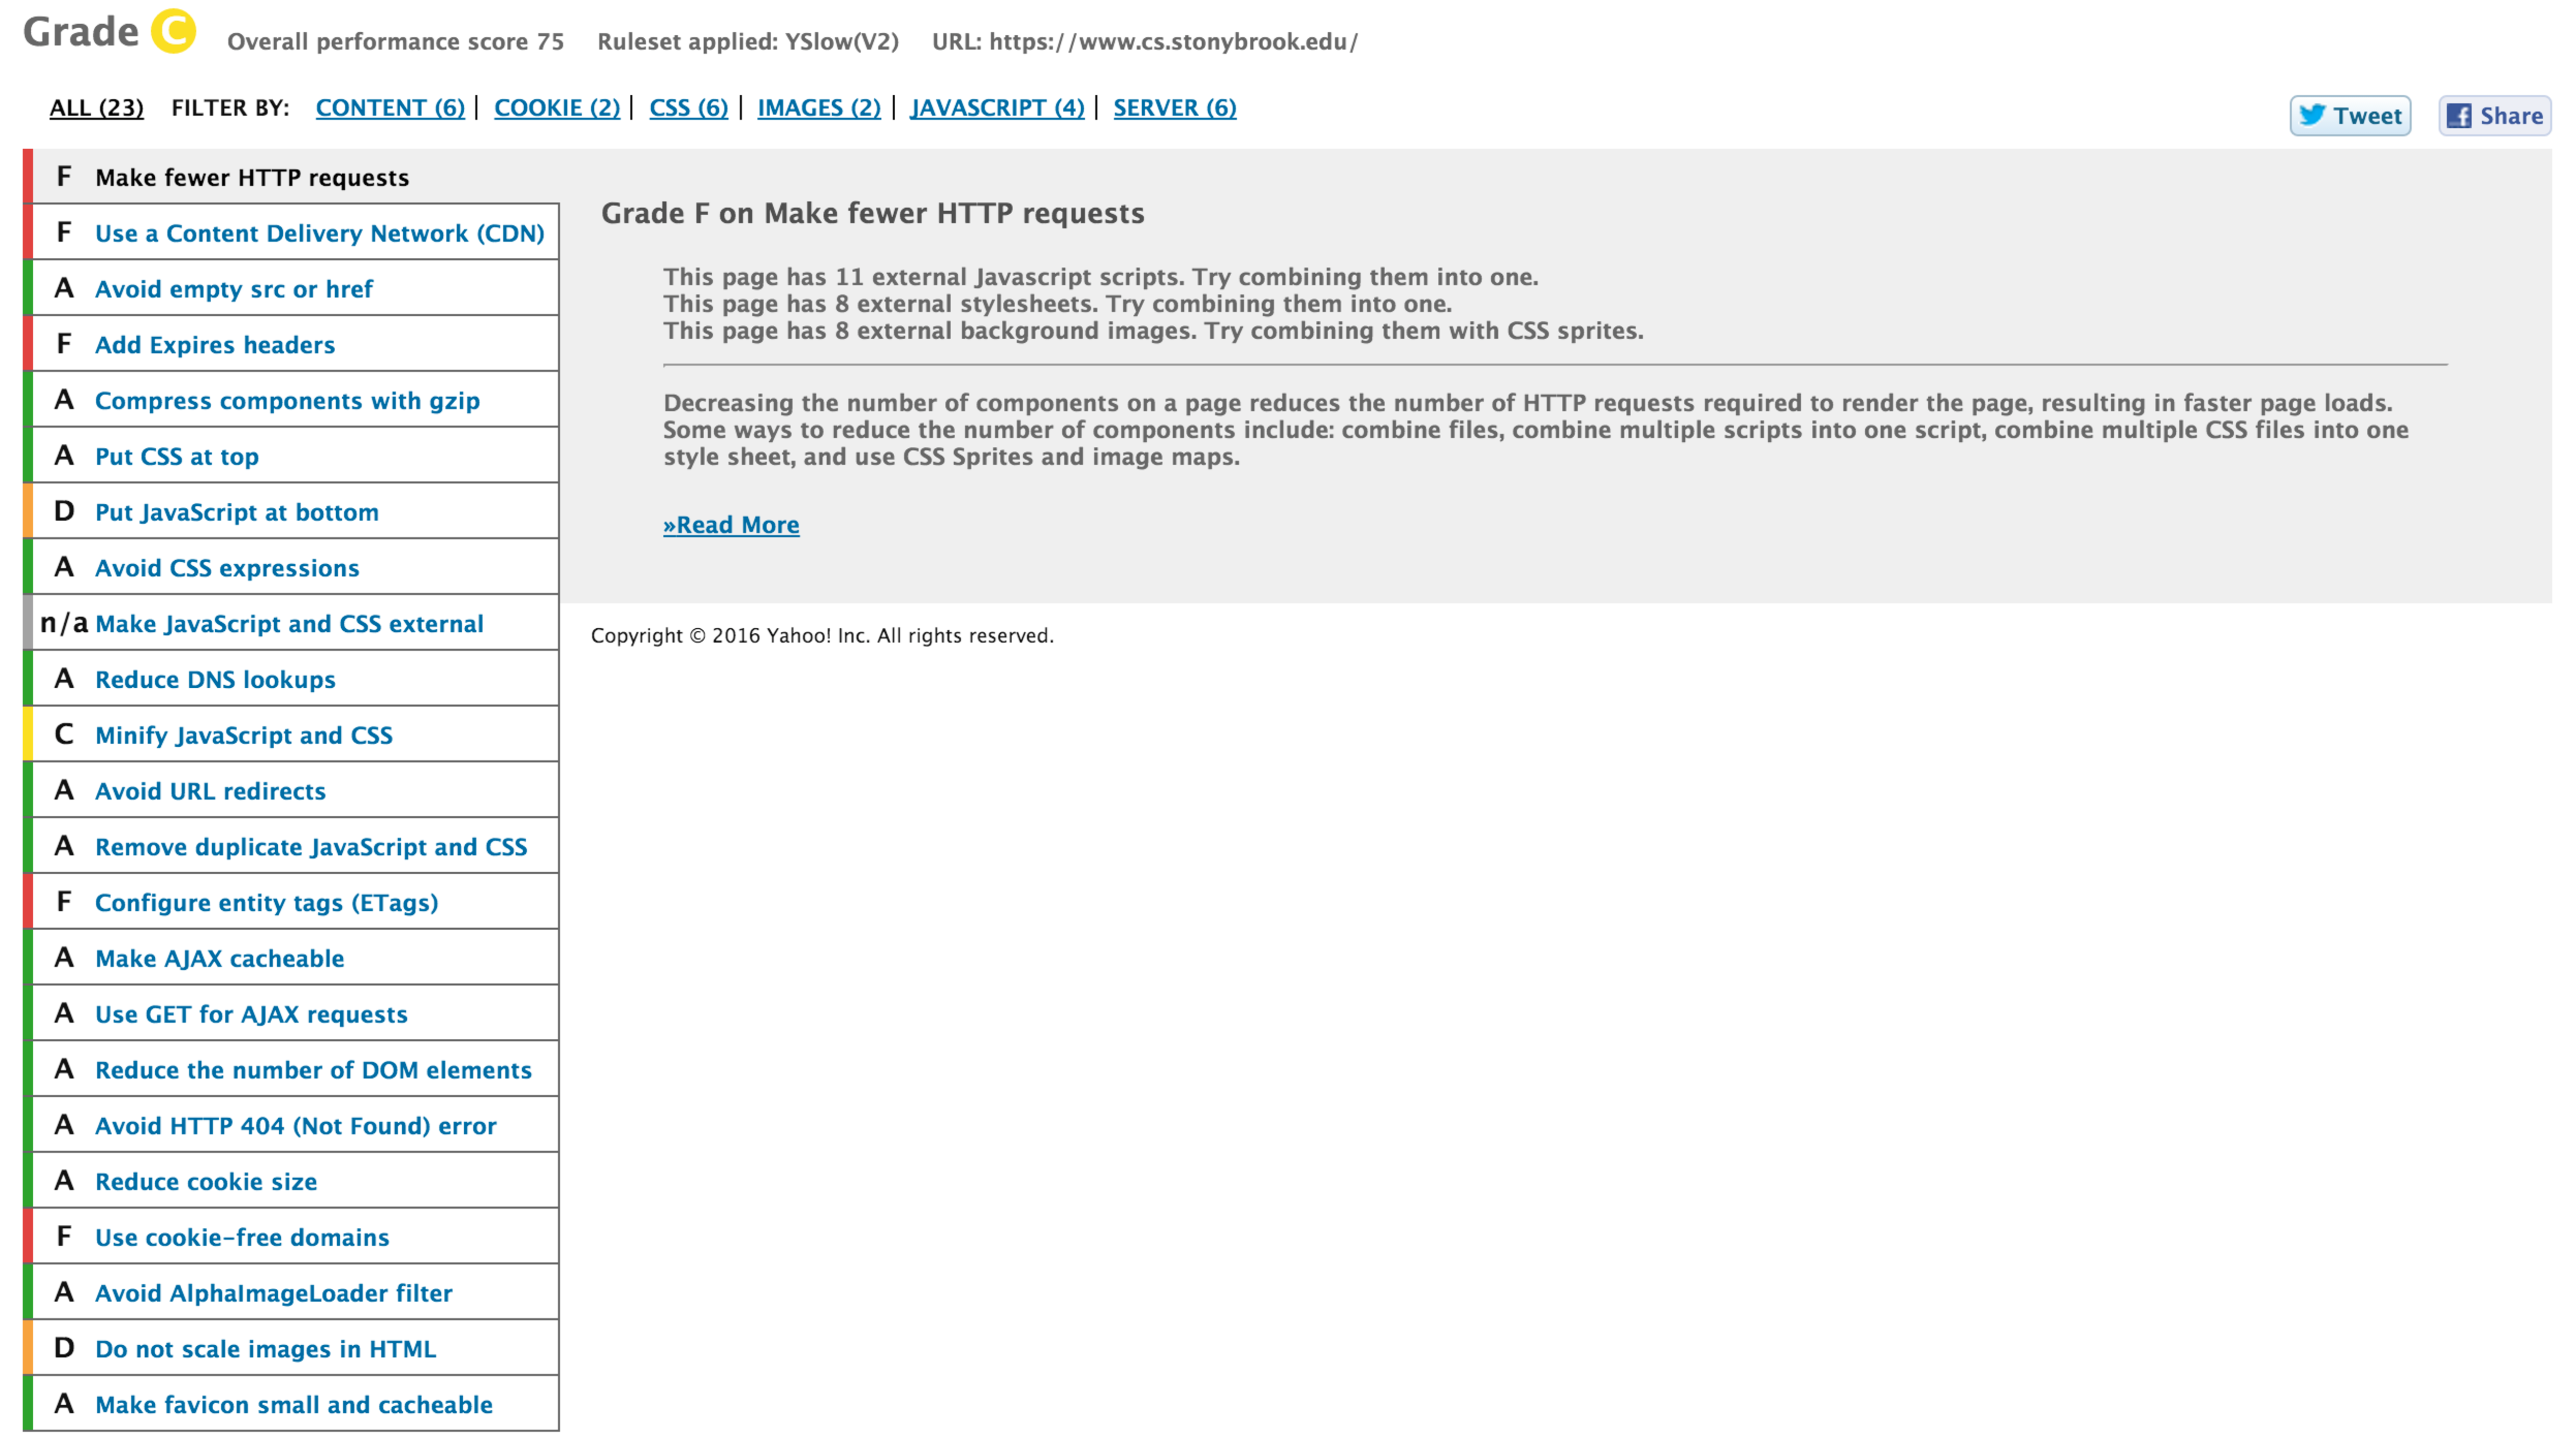
\includegraphics[width=0.85 \textwidth]{./figures/optimization/yslow_stonybrook.pdf}
  \caption {Sample YSLOW analysis for {\em www.cs.stonybrook.edu}}
  \label{fig:yslow_stonybrook}
\end{figure}

\noindent Since YSlow share the same problems with Google's PageSpeed Insight's(Fixed rule sets and unrealistic weights), the optimization results would be similar to the PageSpeed's Insights results.

\section{Our Approach: PLTSpeed}
\noindent In this section, we briefly discuss our approach in which we will score each optimization based on it's contribution to the page load time. We also take into account different network and client conditions when suggesting an optimization.

\subsection{A framework to predict page load time}
 As we have discussed earlier (\S\ref{ch:methodology}), WProf can capture the various activities performed during page load. We analyze these capture files to generate a JSON file for each page load process. Each JSON file contains the timing for all objects in a web page along with their dependencies. A sample snippet of such a JSON file is shown below.
 

 
 \begin{minted}[frame=leftline, framerule=1.5pt, rulecolor=\color{blue}]{json}

 {
   "n_download_no_trigger" : 1,
   "start_activity" : "download_0",
   "name" : "original.testbed.localhost_test4.html",
   "load_activity" : -1,
   "objs" : [
      {
         "when_comp_start" : 1,
         "url" : "http://original.testbed.localhost/test4.html",
         "id" : "r1",
         "comps" : [
            {
               "s_time" : 59.6280004829168,
               "time" : 12.5759998336435,
               "id" : "r1_c1",
               "type" : "evalhtml",
               "e_time" : 72.2040003165603
            },
            {
               "s_time" : 75.6310001015663,
               "time" : 0.867000780999703,
               "type" : "evalhtml",
               "id" : "r1_c2",
               "e_time" : 76.498000882566
            }
         ],
         "download" : {
            "receiveFirst" : 2,
            "len" : 295,
            "dns" : 0,
            "dnsEnd" : -1,
            "receiveHeadersEnd" : 9,
            "sslEnd" : -1,
            "connectEnd" : 6,
            "connectStart" : 0,
            "id" : "download_0",
            "receivedTime" : "11.2190004438162",
            "sslStart" : -1,
            "dnsStart" : -1,
            "receiveLast" : 2.21900044381618,
            "s_time" : 0,
            "sendEnd" : 7,
            "sendStart" : 6,
            "type" : "text/html"
         }
      }
 \end{minted}

 
 
\noindent These JSON files can be seen as structured representation of the whole page load. Now, if we apply an optimization to a Web page, the resulting JSON file will reflect the result of the applied optimization along with new timings and dependencies.\\

\noindent If we had access to the new timings beforehand, we could rewrite the original JSON file and produce the new JSON file. In other words, if we could predict the new computation and download time for each activity involved in a page load process, we were able to rewrite the original JSON file and predict the new page load time after optimizations has been applied.
This process is illustrated in figure \ref{fig:platform}.
\begin{figure}[!htb]
  \centering
    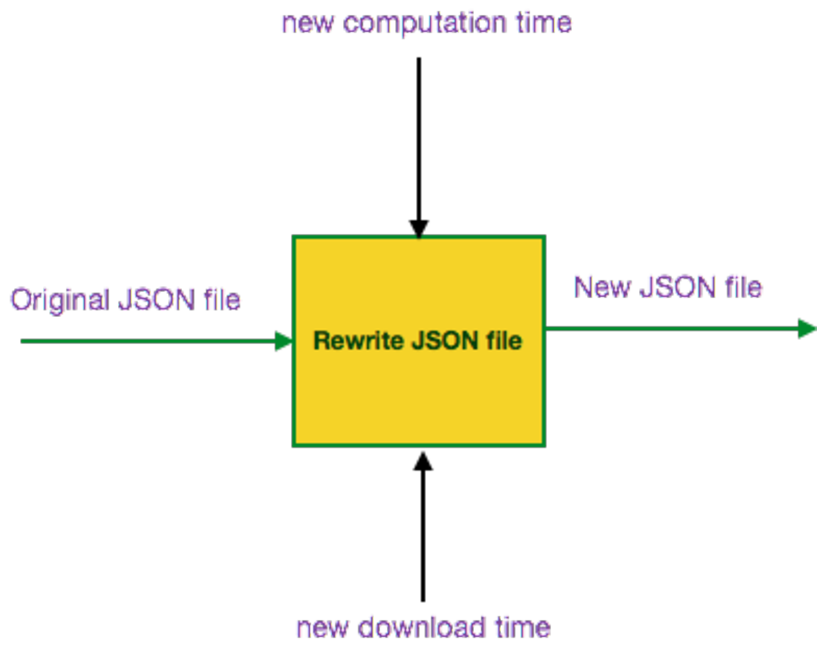
\includegraphics[width=0.85 \textwidth]{./figures/optimization/platform.pdf}
  \caption {Rewriting the original JSON file to predict new page load time.}
  \label{fig:platform}
\end{figure}

\noindent We process each of these new generated JSON files and calculate the critical rendering path. The length of the critical path is the page load time.\\

\subsection {The prediction engine}
To complete our framework from previous section, we now need an infrastructure to predict computation and download times after a certain parameter is changed. This parameter can be applying a new optimization or just a change in connection bandwidth.
 
\noindent For example, to predict new download time after a certain optimization is applied to a Web page, in our testbed, we can apply optimization to lots of locally served web pages. By actually running experiments before and after that optimization, we will be able to model download time for each object present in a page structure.\\
\noindent This model can predict the future network/computation time for each object. This feature (As discussed in previous section) enables us to manipulate the original JSON file and calculate the new critical rendering path time for a particular Web page without applying that particular optimization.

\noindent The block diagram for predicting new download times is depicted in figure \\\ref{fig:predictionengine} 

\begin{figure}[!htb]
  \centering
    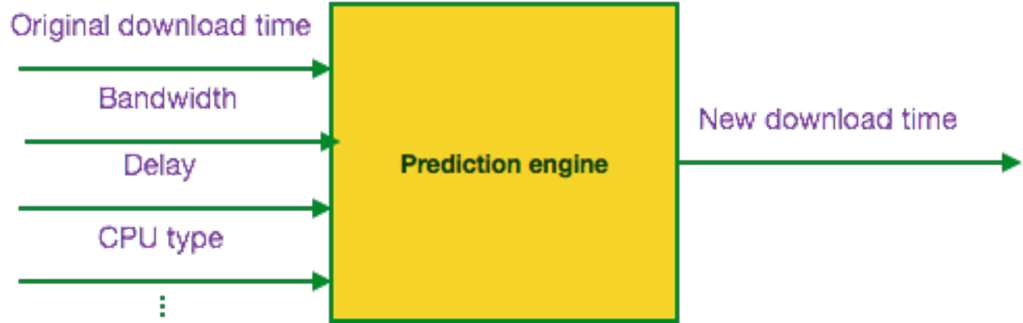
\includegraphics[width=0.85 \textwidth]{./figures/optimization/predictionengine.pdf}
  \caption {Prediction engine}
  \label{fig:predictionengine}
\end{figure}

\noindent We walk through an example to see how computation/networking time can be modeled for a certain type of modification.\\
We apply minification to an external CSS/Javascript and use our testbed to model the impact of this modification. "Minification is the process of removing all unnecessary characters from source code without changing its functionality"\cite{wiki_minification}. \\
The experiment is set up to run an emulated 4G connection. We use Alexa's top 200 web sites and in this case, experiments are run in a desktop environment.
To ignore already minified scripts, we use a simple heuristic which looks for white spaces in the beginning of script source file. If there is no white space, we consider that script as "already minified".\\
The goal is to model computation and network time for minified scripts. We have the timing for all objects in the original web page. Using the testbed, we also have access to the timing for all objects in the new modified web page. This new modified web page has all of it's scripts minified. In order to model how minification affects the computation and networking time, we use linear regression modeling as our prediction algorithm.\\
\noindent In figure \ref{fig:afterbeforeoncp}, the gray bars are length of the original {\em www.youtube.com} (before minification) and the color bars are for minified {\em www.youtube.com}. As we can observe, minification reduces length of objects on critical path in this case and leads to a decreased page load time.
\begin{figure}[!htb]
  \centering
    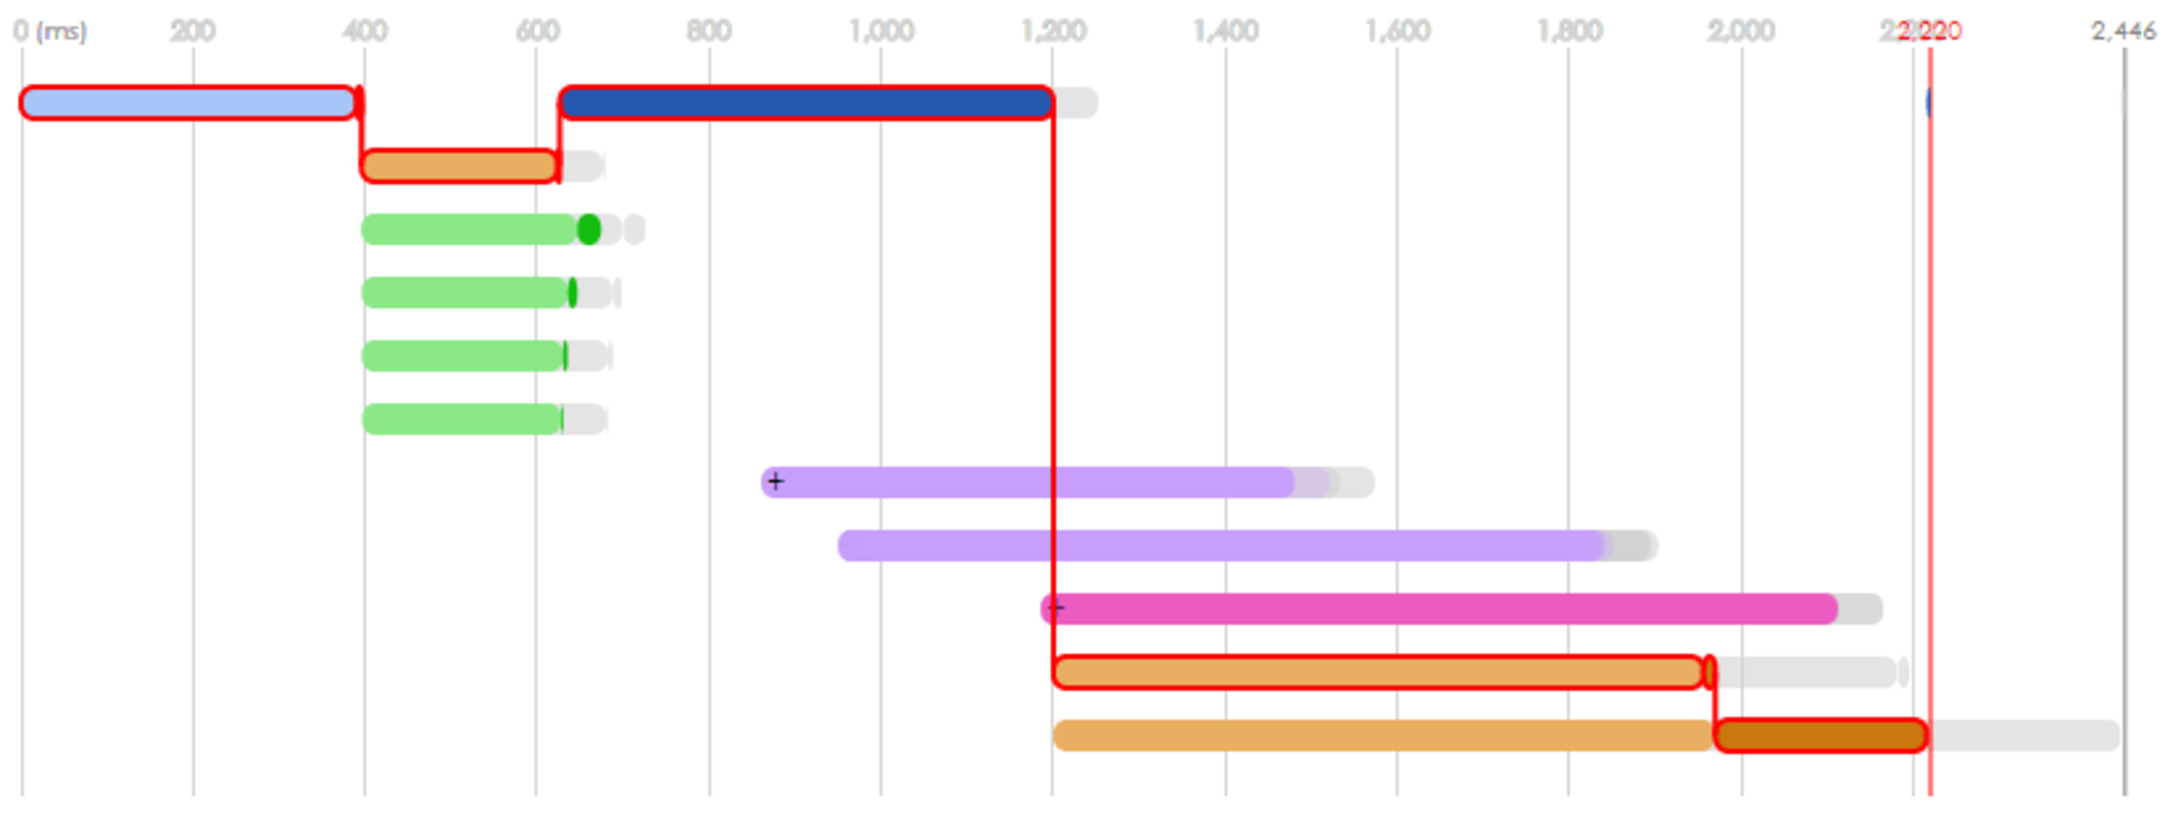
\includegraphics[width=0.85 \textwidth]{./figures/optimization/afterbeforeoncp.pdf}
  \caption {Page load time before/after minification on www.youtube.com}
  \label{fig:afterbeforeoncp}
\end{figure}

\subsection {Future work}
After completing our framework to predict page load time, in future, we will build a web based platform that suggests to users best optimizations applicable to their Web sites. This platform will consider optimization's contribution to page load time along with different networking conditions and user setups.\\
\noindent  One should note that when combining optimizations, the whole gain/loss will not be equal to the sum of all optimizations. Hence, part of our future job will be to study the effect of combination of optimizations. For example, we may observe that minification alone, will improve page load time by 10\% and inlining improves the page load time by 5\% in a certain environment. Obviously we can not conclude that when minification and inlining are both applied to a Web page, we will see overall 15\% improvement in page load time.

%Here we can add d3.js figures for original and modified pages.(Meghna's plots)

%\chapter{PLTSpeed}\label{ch:pltspeed}
A platform to suggest user what improvements they need to apply and the effect of those on PLT
\printbibliography[heading=bibintoc, title={References}]
\label{bib:mybiblio}
%\appendix
%\chapter{Appendix A name}\label{ch:appAlabel}
Here is the first appendix

\end{document}
